\documentclass[]{article}
\usepackage{amssymb,amsmath}
\usepackage{ifxetex,ifluatex}
\ifxetex
  \usepackage{fontspec,xltxtra,xunicode}
  \defaultfontfeatures{Mapping=tex-text,Scale=MatchLowercase}
\else
  \ifluatex
    \usepackage{fontspec}
    \defaultfontfeatures{Mapping=tex-text,Scale=MatchLowercase}
  \else
    \usepackage[utf8]{inputenc}
  \fi
\fi
\usepackage{color}
\usepackage{fancyvrb}
\DefineShortVerb[commandchars=\\\{\}]{\|}
\DefineVerbatimEnvironment{Highlighting}{Verbatim}{commandchars=\\\{\}}
% Add ',fontsize=\small' for more characters per line
\newenvironment{Shaded}{}{}
\newcommand{\KeywordTok}[1]{\textcolor[rgb]{0.00,0.44,0.13}{\textbf{{#1}}}}
\newcommand{\DataTypeTok}[1]{\textcolor[rgb]{0.56,0.13,0.00}{{#1}}}
\newcommand{\DecValTok}[1]{\textcolor[rgb]{0.25,0.63,0.44}{{#1}}}
\newcommand{\BaseNTok}[1]{\textcolor[rgb]{0.25,0.63,0.44}{{#1}}}
\newcommand{\FloatTok}[1]{\textcolor[rgb]{0.25,0.63,0.44}{{#1}}}
\newcommand{\CharTok}[1]{\textcolor[rgb]{0.25,0.44,0.63}{{#1}}}
\newcommand{\StringTok}[1]{\textcolor[rgb]{0.25,0.44,0.63}{{#1}}}
\newcommand{\CommentTok}[1]{\textcolor[rgb]{0.38,0.63,0.69}{\textit{{#1}}}}
\newcommand{\OtherTok}[1]{\textcolor[rgb]{0.00,0.44,0.13}{{#1}}}
\newcommand{\AlertTok}[1]{\textcolor[rgb]{1.00,0.00,0.00}{\textbf{{#1}}}}
\newcommand{\FunctionTok}[1]{\textcolor[rgb]{0.02,0.16,0.49}{{#1}}}
\newcommand{\RegionMarkerTok}[1]{{#1}}
\newcommand{\ErrorTok}[1]{\textcolor[rgb]{1.00,0.00,0.00}{\textbf{{#1}}}}
\newcommand{\NormalTok}[1]{{#1}}
% Redefine labelwidth for lists; otherwise, the enumerate package will cause
% markers to extend beyond the left margin.
\makeatletter\AtBeginDocument{%
  \renewcommand{\@listi}
    {\setlength{\labelwidth}{4em}}
}\makeatother
\usepackage{enumerate}
\usepackage{graphicx}
% We will generate all images so they have a width \maxwidth. This means
% that they will get their normal width if they fit onto the page, but
% are scaled down if they would overflow the margins.
\makeatletter
\def\maxwidth{\ifdim\Gin@nat@width>\linewidth\linewidth
\else\Gin@nat@width\fi}
\makeatother
\let\Oldincludegraphics\includegraphics
\renewcommand{\includegraphics}[1]{\Oldincludegraphics[width=10cm]{#1}}
\ifxetex
  \usepackage[setpagesize=false, % page size defined by xetex
              unicode=false, % unicode breaks when used with xetex
              xetex,
              colorlinks=true,
              linkcolor=blue]{hyperref}
\else
  \usepackage[unicode=true,
              colorlinks=true,
              linkcolor=blue]{hyperref}
\fi
\hypersetup{breaklinks=true, pdfborder={0 0 0}}
\setlength{\parindent}{0pt}
\setlength{\parskip}{6pt plus 2pt minus 1pt}
\setlength{\emergencystretch}{3em}  % prevent overfull lines
\setcounter{secnumdepth}{0}
\usepackage[margin=1.8cm]{geometry}

\author{
Cheshire, James\\
\texttt{james.cheshire@ucl.ac.uk}
\and
Lovelace, Robin\\
\texttt{r.lovelace@leeds.ac.uk}
}
\title{Manipulating and visualizing spatial data with R}

\begin{document}
\maketitle

\section{Introduction}

\subsection{What is R?}

R is a free and open source computer program that runs on all major
operating systems. It relies primarily on the \emph{command line} for
data input: instead of interacting with the program by clicking on
different parts of the screen, so users enter commands via the keyboard.
This will seem to strange to people accustomed to relying on a graphical
user interface (GUI) for most of their computing, yet the approach has a
number of benefits, as highlighted by Gary Sherman (2008, p.~283),
developer of the popular Geographical Information System (GIS) QGIS:

\begin{quote}
With the advent of ``modern'' GIS software, most people want to point
and click their way through life. That's good, but there is a tremendous
amount of flexibility and power waiting for you with the command line.
Many times you can do something on the command line in a fraction of the
time you can do it with a GUI.

\end{quote}
The joy of this, when you get accustomed to it, is that any command is
only ever a few keystrokes away, and the order of the commands sent to R
can be stored and repeated in scripts, saving time in the long-term and
ensuring reproducible results (see ``R and reproducible research'').

Another important attribute of R, related to its command line interface,
is that it is a fully fledged \emph{programming language}. Other GIS
programs are written in lower level languages such as C++ which are kept
at a safe distance from the users by the GUI. In R, by contrast, the
user inputs is the same as what R sees when it processes the request.
Access to R's source code and openness about how it works has enabled a
veritable army of programmers to improve R over time and add an
incredible number of extensions to its capabilities. There are now more
than 4000 official packages for R, allowing it to tackle almost any
computational or numerical problem one could imagine.

Although writing R source code and creating new packages will not appeal
to most R users, it inspires confidence to know that there is a strong
and highly skilled community of R developers. If there is a useful
function that R cannot currently perform, there is a reasonable chance
that someone is working on a solution that will become available at a
later date. One area where extension of R's basic capabilities has been
particularly successful is the addition of a wide variety of spatial
tools.

\subsection{Why R for spatial data visualisation?}

Aside from confusion surrounding its one character name {[}1{]} and
uncertainty about how to search for help {[}2{]}, R may also seem a
strange choice for a tutorial on \emph{spatial} data visualisation
specifically. ``I thought R was just for statistics?'' and ``Why not use
a proper GIS package like ArcGIS?'' are valid questions.

R was conceived - and is still primarily known - for its capabilities as
a ``statistical programming language'' (Bivand and Gebhardt 2000).
Statistical analysis functions remain core to the package but there is a
broadening of functionality to reflect a growing user base across
disciplines. R has become ``an integrated suite of software facilities
for data manipulation, calculation and graphical display'' (Venables et
al. 2013). Spatial data analysis and visualisation is an important
growth area within this increased functionality. In recent years R has
really made its mark as a data visualisation tool. The map of Facebook
friendships produced by Paul Butler is iconic in this regard, and
reached a global audience. He mapped the linkages between friends by
calculating the great circle arcs between them (using the
\texttt{geosphere} package) and plotted the result, displayed in figure
1. The secret to the success of this map was the time taken to select
the appropriate colour palette, line widths and transparency for the
plot. As we discuss in Section 3 the importance of these cannot be
understated and are the difference between a stunning graphic and an
impenetrable mess.

\begin{figure}[htbp]
\centering
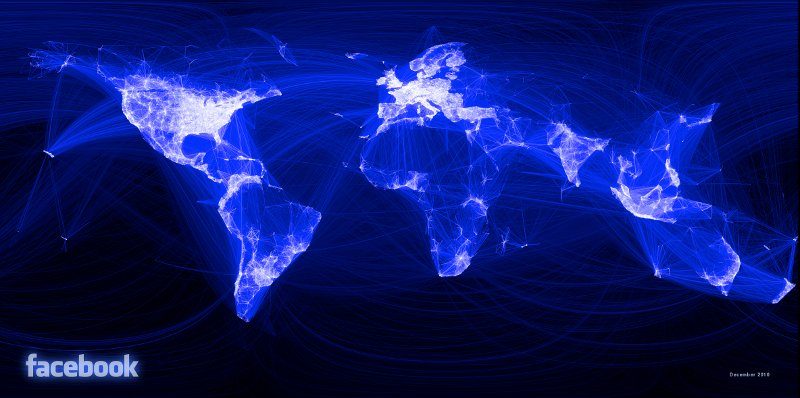
\includegraphics{figure/butler_facebook_2.jpg}
\caption{Iconic plot of Facebook friendship networks worldwide, by Paul
Butler}
\end{figure}

The impact of the graphic was to inspire the R community to produce more
ambitious graphics; a process fuelled by the increased demand for data
visualisation and the development of sophisticated packages, such as
ggplot2, that augment the basic plot functions of R. It is now the case
that R has become a key analysis and visualisation tool used by the
likes of Twitter, the New York Times and Facebook and thousands of
consultants, design houses and journalists. It is not longer the
preserve of academic research, with many graduate jobs listing R as a
desirable skill.

Finally, it is worth noting that while dedicated GIS programs handle
spatial data by default and display the results in a single way, there
are various options in R that must be decided by the user, for example
whether to use R's base graphics or a dedicated graphics package such as
ggplot2. On the other hand, the main benefits of R for spatial data
visualisation lie in the \emph{reproducibility} of its outputs, a
feature that we will be using to great effect in this tutorial.

\subsubsection{R and reproducible research}

There is a drive towards transparency in data and methods datasets in
academic publishing. R encourages truly transparent and reproducible
research by enabling anyone with an R installation reproduce results
described in a previous paper. This process is eased by the RStudio
integrated development environment (IDE) that allows `live' R code and
results to be embedded in documents. In fact, this tutorial was written
in RStudio and can be recompiled on any computer by downloading the
project's GitHub repository.

\subsection{Getting started with the tutorial}

The first stage with this tutorial is to download the data from GitHub,
where an updated version is stored:
\href{https://github.com/geocomPP/sdvwR}{github.com/geocomPP/sdvwR}.
Click on the ``Download ZIP'' button on the right, and unpack the folder
to a sensible place on your computer (e.g.~the Desktop). Explore the
folder and try opening some of the files, especially those from the
sub-folder entitled ``data'': these are the input datasets we'll be
using.

For the purpose of this practical we will be using the RStudio software
installed on a server. This marks a real step forward in terms of the
use of R ``in the cloud'' by enabling users to access the software from
their web browser. This is the first time we have tried this so lets
hope it goes smoothly!

In Firefox go to http://marlin.casa.ucl.ac.uk/rstudio (this is only
accessible if you are part of the UCL network). Enter the log in details
you have been given and you should see the RStudio interface. In the
bottom right window you should see an ``Upload'' button. Click on this
and upload the zipfile you have just downloaded from github. RStudio
will automatically uncompress this and you should see the list of files
and folders appear. At the end of today you can tick the boxes next to
the files/ folders you want and then under the ``More'' menu export them
to a zipfile that you can email to yourself or take on a memory stick.

\section{R and Spatial Data}

\subsection{Preliminaries}

R has a unique syntax that is worth learning in basic terms before
loading spatial data: to R spatial and non-spatial data are treated in
the same way, although they have different underlying data structures.

The first step is to ensure that you are in the correct working
directory. Use \texttt{setwd} to select the correct folder. Assuming the
folder has been downloaded from GitHub and unpacked into the desktop on
a Windows computer, you would type the following:

\begin{Shaded}
\begin{Highlighting}[]
\KeywordTok{setwd}\NormalTok{(}\StringTok{"C:/Users/Uname/Desktop/sdvwR-master"}\NormalTok{)}
\end{Highlighting}
\end{Shaded}
In RStudio, it is recommended to work from \emph{script files}. To open
a new R script, click \texttt{File \textgreater{} New File} (see the
\href{http://www.rstudio.com/ide/docs/using/keyboard\_shortcuts}{RStudio
website} for shortcuts.) Try typing and running (by pressing
\texttt{ctl-Enter} in an RStudio script) the following calculations to
see how R works and plot the result.

\begin{Shaded}
\begin{Highlighting}[]
\NormalTok{t <- }\KeywordTok{seq}\NormalTok{(}\DataTypeTok{from =} \DecValTok{0}\NormalTok{, }\DataTypeTok{to =} \DecValTok{20}\NormalTok{, }\DataTypeTok{by =} \FloatTok{0.1}\NormalTok{)}
\NormalTok{x <- }\KeywordTok{sin}\NormalTok{(t) * }\KeywordTok{exp}\NormalTok{(-}\FloatTok{0.2} \NormalTok{* t)}
\KeywordTok{plot}\NormalTok{(t, x)}
\end{Highlighting}
\end{Shaded}
\begin{figure}[htbp]
\centering
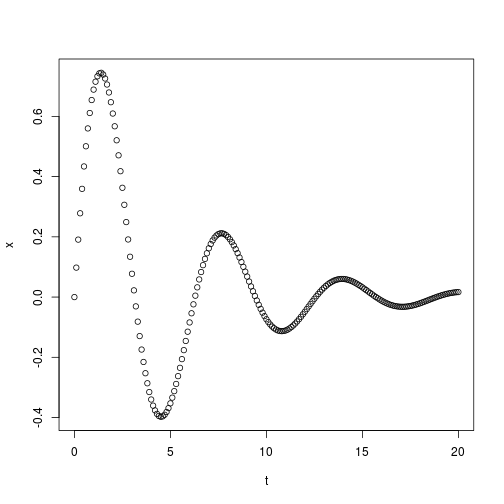
\includegraphics{figure/A_preliminary_plot.png}
\caption{A preliminary plot}
\end{figure}

R code consists of \emph{functions}, usually proceeded by brackets (e.g.
\texttt{seq}) and \emph{objects} (\texttt{d}, \texttt{t} and
\texttt{x}). Each function contains \emph{arguments}, the names of which
often do not need to be stated: the function \texttt{seq(0, 20, 0.1)},
for example, would also work because \texttt{from}, \texttt{to} and
\texttt{by} are the \emph{default} arguments. Knowing this is important
as it can save typing. In this tutorial, however, we generally spell out
each of the argument names, for clarity.

Note the use of the assignment arrow \texttt{\textless{}-} to create new
objects. Objects are entities that can be called to by name in R and can
be renamed through additional assignements (e.g
\texttt{y \textless{}- x} if y seems a more appropriate name). This is
an efficient way of referring to large data objects or sets of commands.

\subsection{Spatial Data in R}

In any data analysis project, spatial or otherwise, it is important to
have a strong understanding of the dataset before progressing. This
section will therefore begin with a description of the input data. We
will see how data can be loaded into R and exported to other formats,
before going into more detail about the underlying structure of spatial
data in R.

\subsubsection{Loading spatial data in R}

In most situations, the starting point of a spatial analysis project is
to load in the datasets. These may originate from government agencies,
remote sensing devices or `volunteered geographical information'
(Goodchild 2007). R is able to import a very wide range of spatial data
formats thanks to its interface with the Geospatial Data Abstraction
Library (GDAL), which is enabled by the package \texttt{rgdal}. Below we
will install the rgdal package using the function
\texttt{install.packages} (this can be used to install any packages) and
then load data from two spatial data formats: GPS eXchange
(\texttt{.gpx}) and ESRI's Shapefile.

\texttt{readOGR} is in fact capable of loading dozens more file formats,
so the focus is on the \emph{method} rather than the specific formats.
Let's start with a \texttt{.gpx} file, a tracklog recording a bicycle
ride from Sheffield to Wakefield uploaded OpenStreetMap {[}3{]}.

\begin{Shaded}
\begin{Highlighting}[]
\KeywordTok{install.packages}\NormalTok{(}\StringTok{"rgdal"}\NormalTok{)}
\end{Highlighting}
\end{Shaded}
\begin{verbatim}
## Error: trying to use CRAN without setting a mirror
\end{verbatim}
\begin{Shaded}
\begin{Highlighting}[]
\KeywordTok{library}\NormalTok{(rgdal)  }\CommentTok{# load the gdal package}
\KeywordTok{ogrListLayers}\NormalTok{(}\DataTypeTok{dsn =} \StringTok{"data/gps-trace.gpx"}\NormalTok{)}
\NormalTok{shf2lds <- }\KeywordTok{readOGR}\NormalTok{(}\DataTypeTok{dsn =} \StringTok{"data/gps-trace.gpx"}\NormalTok{, }\DataTypeTok{layer =} \StringTok{"tracks"}\NormalTok{)  }\CommentTok{# load track}
\KeywordTok{plot}\NormalTok{(shf2lds)}
\NormalTok{shf2lds.p <- }\KeywordTok{readOGR}\NormalTok{(}\DataTypeTok{dsn =} \StringTok{"data/gps-trace.gpx"}\NormalTok{, }\DataTypeTok{layer =} \StringTok{"track_points"}\NormalTok{)  }\CommentTok{# load points}
\KeywordTok{points}\NormalTok{(shf2lds.p[}\KeywordTok{seq}\NormalTok{(}\DecValTok{1}\NormalTok{, }\DecValTok{3000}\NormalTok{, }\DecValTok{100}\NormalTok{), ])}
\end{Highlighting}
\end{Shaded}
\begin{figure}[htbp]
\centering
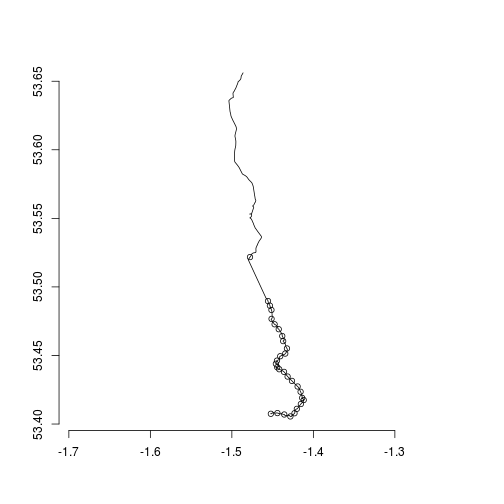
\includegraphics{figure/Leeds_to_Sheffield_GPS_data.png}
\caption{Leeds to Sheffield GPS data}
\end{figure}

In the code above we first used R to \emph{download} a file from the
internet, using the function \texttt{download.file} (note this has been
\emph{commented out} using the \texttt{\#} symbol). The two essential
arguments of this function are \texttt{url} (we could have typed
\texttt{url =} before the link) and \texttt{destfile}, the destination
file. As with any function, more optional arguments can be viewed by by
typing \texttt{?download.file}.

When \texttt{rgdal} has successfully loaded, the next task is not to
import the file directly, but to find out which \emph{layers} are
available to import, with \texttt{ogrListLayers}. The output from this
command tells us that various layers are available, including
\texttt{tracks} and \texttt{track\_points}. These are imported into R's
\emph{workspace} using \texttt{readOGR}.

Finally, the basic \texttt{plot} function is used to visualize the newly
imported objects, ensuring they make sense. In the second plot function
(\texttt{points}), we add points for a subset of the object. There will
be no axes in the plot; to see how to add them, enter \texttt{?axis}

Try discovering more about the function by typing \texttt{?readOGR}. The
documentation explains that the \texttt{dsn =} argument is interpreted
differently depending on the type of file used. In the above example,
the \texttt{dsn} was set to as the name of the file. To load Shapefiles,
by contrast, the \emph{folder} containing the data is used:

\begin{Shaded}
\begin{Highlighting}[]
\NormalTok{lnd <- }\KeywordTok{readOGR}\NormalTok{(}\DataTypeTok{dsn =} \StringTok{"data/"}\NormalTok{, }\StringTok{"london_sport"}\NormalTok{)}
\end{Highlighting}
\end{Shaded}
Here, the files reside in a folder entitled \texttt{data}, which is in
R's current working directory (you can check this using
\texttt{getwd()}). If the files were stored in the working directory,
one would use \texttt{dsn = "."} instead. Again, it may be wise to plot
the data that results, to ensure that it has worked correctly. Now that
the data has been loaded into R's own \texttt{sp} format, try
interrogating and plotting it, using functions such as \texttt{summary}
and \texttt{plot}.

The london\_sport file contains data pertaining to the percentage of
people within each London Borough who regularly undertake physical
activity and also the 2001 population of each Borough.

\subsubsection{The size of spatial datasets in R}

Any datasets that have been read into R's \emph{workspace}, which
constitutes all objects that can be accessed by name and can be listed
using the \texttt{ls()} function, can be saved in R's own data storage
file type \texttt{.RData}. Spatial datasets can get quite large and this
can cause problems on computers by consuming all available memory (RAM)
or hard disk space. It is therefore wise to understand roughly how large
spatial objects are, providing insight into how long certain functions
will take to run.

In the absence of prior knowledge, which of the two objects loaded in
the previous section would one expect to be larger? One could
hypothesize that the London dataset would be larger based on its greater
spatial extent, but how much larger? The answer in R is found in the
function \texttt{object.size}:

\begin{Shaded}
\begin{Highlighting}[]
\KeywordTok{object.size}\NormalTok{(shf2lds)}
\end{Highlighting}
\end{Shaded}
\begin{verbatim}
## 107464 bytes
\end{verbatim}
\begin{Shaded}
\begin{Highlighting}[]
\KeywordTok{object.size}\NormalTok{(lnd)}
\end{Highlighting}
\end{Shaded}
\begin{verbatim}
## 125544 bytes
\end{verbatim}
In fact, the objects have similar sizes: the GPS dataset is surprisingly
large. To see why, we can find out how many \emph{vertices} (points
connected by lines) are contained in each dataset. To do this we use
\texttt{fortify} from the ggplot2 package (use the same method used for
rgdal, described above, to install it).

\begin{Shaded}
\begin{Highlighting}[]
\NormalTok{shf2lds.f <- }\KeywordTok{fortify}\NormalTok{(shf2lds)}
\KeywordTok{nrow}\NormalTok{(shf2lds.f)}
\end{Highlighting}
\end{Shaded}
\begin{verbatim}
## [1] 6085
\end{verbatim}
\begin{Shaded}
\begin{Highlighting}[]

\NormalTok{lnd.f <- }\KeywordTok{fortify}\NormalTok{(lnd)}
\end{Highlighting}
\end{Shaded}
\begin{verbatim}
## Regions defined for each Polygons
\end{verbatim}
\begin{Shaded}
\begin{Highlighting}[]
\KeywordTok{nrow}\NormalTok{(lnd.f)}
\end{Highlighting}
\end{Shaded}
\begin{verbatim}
## [1] 1102
\end{verbatim}
In the above block of code we performed two functions for each object:
1) \emph{flatten} the dataset so that each vertice is allocated a unique
row 2) use \texttt{nrow} to count the result.

It is clear that the GPS data has almost 6 times the number of vertices
compared to the London data, explaining its large size. Yet when
plotted, the GPS data does not seem more detailed, implying that some of
the vertices in the object are not needed for effective visualisation
since the nodes of the line are imperceptible.

\subsubsection{Simplifying geometries}

Simplifcation can help to make a graphic more readable and less
cluttered. Within the `rgeos' package it is possible to use the
\texttt{gSimplify} function to simplify spatial R objects:

\begin{Shaded}
\begin{Highlighting}[]
\KeywordTok{library}\NormalTok{(rgeos)}
\NormalTok{shf2lds.simple <- }\KeywordTok{gSimplify}\NormalTok{(shf2lds, }\DataTypeTok{tol =} \FloatTok{0.001}\NormalTok{)}
\NormalTok{(}\KeywordTok{object.size}\NormalTok{(shf2lds.simple)/}\KeywordTok{object.size}\NormalTok{(shf2lds))[}\DecValTok{1}\NormalTok{]}
\end{Highlighting}
\end{Shaded}
\begin{verbatim}
## [1] 0.04608
\end{verbatim}
\begin{Shaded}
\begin{Highlighting}[]
\KeywordTok{plot}\NormalTok{(shf2lds.simple)}
\KeywordTok{plot}\NormalTok{(shf2lds, }\DataTypeTok{col =} \StringTok{"red"}\NormalTok{, }\DataTypeTok{add =} \NormalTok{T)}
\end{Highlighting}
\end{Shaded}
In the above block of code, \texttt{gSimplify} is given the object
\texttt{shf2lds} and the \texttt{tol} argument of 0.001 (much larger
tolerance values may be needed, for data that is \emph{projected}).
Next, we divide the size of the simplified object by the original (note
the use of the \texttt{/} symbol). The output of \texttt{0.04...} tells
us that the new object is only around 4\% of its original size. We can
see how this has happened by again counting the number of vertices. This
time we use the \texttt{coordinates} and \texttt{nrow} functions
together:

\begin{Shaded}
\begin{Highlighting}[]
\KeywordTok{nrow}\NormalTok{(}\KeywordTok{coordinates}\NormalTok{(shf2lds.simple)[[}\DecValTok{1}\NormalTok{]][[}\DecValTok{1}\NormalTok{]])}
\end{Highlighting}
\end{Shaded}
\begin{verbatim}
## [1] 44
\end{verbatim}
The syntax of the double square brackets will seem strange, providing a
taster of how R `sees' spatial data. Do not worry about this for now. Of
interest here is that the number of vertices has shrunk, from over 6,000
to only 44, without losing much information about the shape of the line.
To test this, try plotting the original and simplified tracks on your
computer: when visualized using the \texttt{plot} function, object
\texttt{shf2lds.simple} retains the overall shape of the line and is
virtually indistinguishable from the original object.

This example is rather contrived because even the larger object
\texttt{shf2lds} is only a tenth of a megabyte, negligible compared with
the gigabytes of memory available to modern computers. However, it
underlines a wider point: for visualizing \emph{small scale} maps,
spatial data \emph{geometries} can often be simplified to reduce
processing time and use of memory.

\subsubsection{Saving and exporting spatial objects}

A typical R workflow involves loading the data, processing/analysing the
data and finally exporting the data in a new form. \texttt{writeOGR},
the logical counterpart of \texttt{readOGR} is ideal for this task. This
is performed using the following command (in this case we are exporting
to an ESRI Shapefile):

\begin{Shaded}
\begin{Highlighting}[]
\NormalTok{shf2lds.simple <- }\KeywordTok{SpatialLinesDataFrame}\NormalTok{(shf2lds.simple, }\KeywordTok{data.frame}\NormalTok{(}\DataTypeTok{row.names =} \StringTok{"0"}\NormalTok{, }
    \DataTypeTok{a =} \DecValTok{1}\NormalTok{))}
\KeywordTok{writeOGR}\NormalTok{(shf2lds.simple, }\DataTypeTok{layer =} \StringTok{"shf2lds"}\NormalTok{, }\DataTypeTok{dsn =} \StringTok{"data/"}\NormalTok{, }\DataTypeTok{driver =} \StringTok{"ESRI Shapefile"}\NormalTok{)}
\end{Highlighting}
\end{Shaded}
In the above code, the object was first converted into a spatial
dataframe class required by the \texttt{writeOGR} command, before being
exported as a shapefile entitled shf2lds. Unlike with \texttt{readOGR},
the driver must be specified, in this case with ``ESRI Shapefile''
{[}4{]}. The simplified GPS data are now available to other GIS programs
for further analysis. Alternatively,
\texttt{save(shf2lds.simple, file = "data/shf2lds.RData")} will save the
object in R's own spatial data format, which is described in the next
section.

\subsubsection{The structure of spatial data in R}

Spatial datasets in R are saved in their own format, defined as
\texttt{Spatial...} classes within the \texttt{sp} package. For this
reason, \texttt{sp} is the basic spatial package in R, upon which the
others depend. Spatial classes range from the basic \texttt{Spatial}
class to the complex \texttt{SpatialPolygonsDataFrame}: the
\texttt{Spatial} class contains only two required \emph{slots} {[}5{]}:

\begin{Shaded}
\begin{Highlighting}[]
\KeywordTok{getSlots}\NormalTok{(}\StringTok{"Spatial"}\NormalTok{)}
\end{Highlighting}
\end{Shaded}
\begin{verbatim}
##        bbox proj4string 
##    "matrix"       "CRS"
\end{verbatim}
This tells us that \texttt{Spatial} objects must contain a bounding box
(\texttt{bbox}) and a coordinate reference system (CRS) accessed via the
function \texttt{proj4string}. Further details on these can be found by
typing \texttt{?bbox} and \texttt{?proj4string}. All other spatial
classes in R build on this foundation of a bounding box and a projection
system (which is set automatically to \texttt{NA} if it is not known).
However, more complex classes contain more slots, some of which are
lists which contain additional lists. To find out the slots of
\texttt{shf2lds.simple}, for example, we would first ascertain its class
and then use the \texttt{getSlots} command:

\begin{Shaded}
\begin{Highlighting}[]
\KeywordTok{class}\NormalTok{(shf2lds.simple)  }\CommentTok{# identify the object's class}
\end{Highlighting}
\end{Shaded}
\begin{verbatim}
## [1] "SpatialLinesDataFrame"
## attr(,"package")
## [1] "sp"
\end{verbatim}
\begin{Shaded}
\begin{Highlighting}[]
\KeywordTok{getSlots}\NormalTok{(}\StringTok{"SpatialLinesDataFrame"}\NormalTok{)  }\CommentTok{# find the associated slots}
\end{Highlighting}
\end{Shaded}
\begin{verbatim}
##         data        lines         bbox  proj4string 
## "data.frame"       "list"     "matrix"        "CRS"
\end{verbatim}
The same principles apply to all spatial classes including
\texttt{Spatial* Points}, \texttt{Polygons} \texttt{Grids} and
\texttt{Pixels} as well as associated \texttt{*DataFrame} classes. For
more information on this, see the \texttt{sp} documentation:
\texttt{?Spatial}.

\subsection{Manipulating spatial data}

\subsubsection{Coordinate reference systems}

As mentioned in the previous section, all \texttt{Spatial} objects in R
are allocated a coordinate reference system (CRS). The CRS of any
spatial object can be found using the command \texttt{proj4string}. In
some cases the CRS is not known: in this case the result will simply be
\texttt{NA}. To discover the CRS of the \texttt{lnd} object for example,
type the following:

\begin{Shaded}
\begin{Highlighting}[]
\KeywordTok{proj4string}\NormalTok{(lnd)}
\end{Highlighting}
\end{Shaded}
\begin{verbatim}
## [1] "+proj=tmerc +lat_0=49 +lon_0=-2 +k=0.9996012717 +x_0=400000 +y_0=-100000 +ellps=airy "
\end{verbatim}
The output may seem cryptic, but is in fact highly informative:
\texttt{lnd} has \emph{projected} coordinates, based on the
\href{http://en.wikipedia.org/wiki/Transverse\_Mercator\_projection}{\emph{Transverse
Mercator}} system (hence \texttt{"+proj=tmerc"} in the output) and its
origin is at latitude 49N, -2E.

If we \emph{know} that the CRS is incorrectly specified, it can be
re-set. In this case, for example we know that \texttt{lnd} actually has
a CRS of OSGB1936. Knowing also that the code for this is 27700, it can
be updated as follows:

\begin{Shaded}
\begin{Highlighting}[]
\KeywordTok{proj4string}\NormalTok{(lnd) <- }\KeywordTok{CRS}\NormalTok{(}\StringTok{"+init=epsg:27700"}\NormalTok{)}
\KeywordTok{proj4string}\NormalTok{(lnd)}
\end{Highlighting}
\end{Shaded}
\begin{verbatim}
## [1] "+init=epsg:27700 +proj=tmerc +lat_0=49 +lon_0=-2 +k=0.9996012717 +x_0=400000 +y_0=-100000 +datum=OSGB36 +units=m +no_defs +ellps=airy +towgs84=446.448,-125.157,542.060,0.1502,0.2470,0.8421,-20.4894"
\end{verbatim}
The CRS has now been updated - note that the key details are all the
same as before. Note: this method should \textbf{never} be used as an
attempt to \emph{reproject} data from one CRS to another.

\subsubsection{Reprojecting data}

Transforming the coordinates of spatial data from one CRS to another
(reprojection) is a common task in GIS. This is because data from
national sources are generally provided in \emph{projected} coordinates
(the location on the cartesian coordinates of a map) whereas data from
GPSs and the internet are generally provided in \emph{geographic}
coordinates, with latitude and longitude measured in degrees to locate
points on the surface of the globe.

Reprojecting data in R is quite simple: all you need is a spatial object
with a known CRS and knowledge of the CRS you wish to transform it to.
To illustrate why that is necessary, try to plot the objects
\texttt{lnd} and \texttt{shf2lnd.simple} on the same map:

\begin{Shaded}
\begin{Highlighting}[]
\NormalTok{combined <- }\KeywordTok{rbind}\NormalTok{(}\KeywordTok{fortify}\NormalTok{(shf2lds.simple)[, }\DecValTok{1}\NormalTok{:}\DecValTok{2}\NormalTok{], }\KeywordTok{fortify}\NormalTok{(lnd)[, }\DecValTok{1}\NormalTok{:}\DecValTok{2}\NormalTok{])}
\KeywordTok{plot}\NormalTok{(combined)}
\end{Highlighting}
\end{Shaded}
\begin{figure}[htbp]
\centering
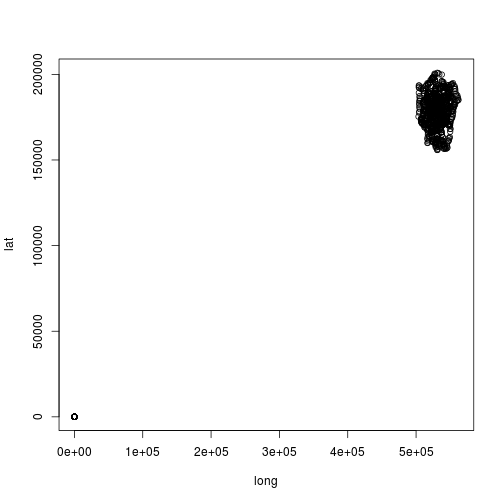
\includegraphics{figure/Plot_of_spatial_objects_with_different_CRS.png}
\caption{Plot of spatial objects with different CRS}
\end{figure}

In the above code we first extracted the coordinates of the vertices of
each line and polygon using \texttt{fortify} and then plotted them using
\texttt{plot}. The image shows why reprojection is necessary: the
\texttt{.gpx} data are on a totally different scale than the shapefile
of London. Hence the tiny dot at the bottom left of the graph. We will
now reproject the data, allowing \texttt{lnd} and
\texttt{shf2lds.simple} to be usefully plotted on the same graphic:

\begin{Shaded}
\begin{Highlighting}[]
\NormalTok{lnd.wgs84 <- }\KeywordTok{spTransform}\NormalTok{(lnd, }\DataTypeTok{CRSobj =} \KeywordTok{CRS}\NormalTok{(}\StringTok{"+init=epsg:4326"}\NormalTok{))}
\end{Highlighting}
\end{Shaded}
The above code created a new object,\texttt{lnd.wgs84}, that contains
the same geometries as the original but in a new CRS using the
\texttt{spTransform} function. The \texttt{CRS} argument was set to
\texttt{"+init=epsg:4326"}, which represents the WGS84 CRS via an EPSG
code {[}6{]}. Now \texttt{lnd} has been reprojected we can plot it next
to the GPS data:

\begin{Shaded}
\begin{Highlighting}[]
\NormalTok{combined <- }\KeywordTok{rbind}\NormalTok{(}\KeywordTok{fortify}\NormalTok{(shf2lds.simple)[, }\DecValTok{1}\NormalTok{:}\DecValTok{2}\NormalTok{], }\KeywordTok{fortify}\NormalTok{(lnd.wgs84)[, }\DecValTok{1}\NormalTok{:}\DecValTok{2}\NormalTok{])}
\KeywordTok{plot}\NormalTok{(combined)}
\end{Highlighting}
\end{Shaded}
\begin{figure}[htbp]
\centering
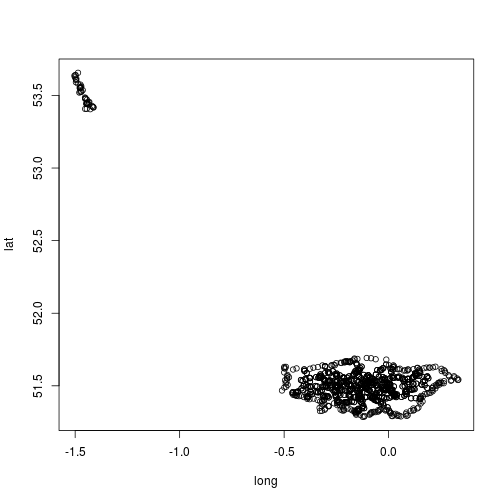
\includegraphics{figure/Plot_of_spatial_objects_sharing_the_same_CRS.png}
\caption{Plot of spatial objects sharing the same CRS}
\end{figure}

Although the plot of the reprojected data is squashed because the axis
scales are not fixed and distorted (\emph{geographic} coordinates such
as WGS84 distort space close to the poles), but at least the relative
position and shape of both objects can now be seen (making
visualisations attractive is covered in the next major section). The
presence of the dotted line in the top left of the plot confirms our
assumption that the GPS data is from around Sheffield, which is
northwest of London.

\subsubsection{Attribute joins}

London Boroughs are official administrative zones so we can easily join
a range of other datasets to the polygons in the \texttt{lnd} object. We
will use the example of crime data to illustrate this data availability,
which is stored in the \texttt{data} folder available from this
project's github page.

\begin{Shaded}
\begin{Highlighting}[]
\KeywordTok{load}\NormalTok{(}\StringTok{"data/crimeAg.Rdata"}\NormalTok{)  }\CommentTok{# load the crime dataset from an R dataset}
\end{Highlighting}
\end{Shaded}
After the dataset has been explored (e.g.~using the \texttt{summary} and
\texttt{head} functions) to ensure compatibility, it can be joined to
\texttt{lnd}. We will use the the \texttt{join} function in the
\texttt{plyr} package but the \texttt{merge} function could equally be
used (remember to type \texttt{library(plyr)} if needed).

\texttt{join} requires all joining variables to have the same name,
which has already been done {[}7{]}.

\begin{Shaded}
\begin{Highlighting}[]
\NormalTok{lnd@data <- }\KeywordTok{join}\NormalTok{(lnd@data, crimeAg)}
\end{Highlighting}
\end{Shaded}
Take a look at the \texttt{lnd@data} object. You should see new
variables added, meaning the attribute join was successful.

\subsection{Spatial joins}

A spatial join, like an attribute join, is used to transfer information
from one dataset to another. There is a clearly defined direction to
spatial joins, with the \emph{target layer} receiving information from
another spatial layer based on the proximity of elements from both
layers to each other. There are three broad types of spatial join:
one-to-one, many-to-one and one-to-many. We will focus only the former
two as the third type is rarely used.

\subsubsection{One-to-one spatial joins}

One-to-one spatial joins are by far the easiest to understand and
compute because they simply involve the transfer of attributes in one
layer to another, based on location. A one-to-one join is depicted in
Figure 6 below, and can performed using the same technique as described
in the section on spatial aggregation.

\begin{figure}[htbp]
\centering
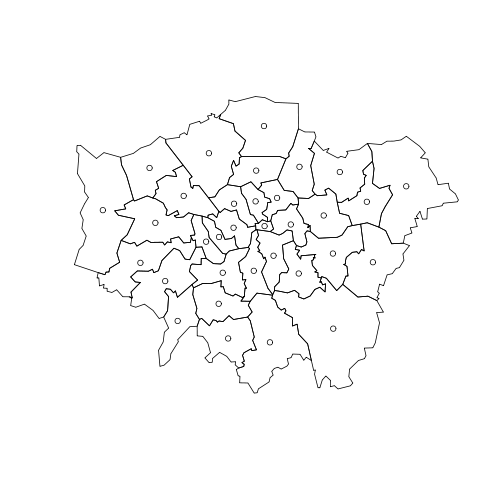
\includegraphics{figure/Illustration_of_a_one-to-one_spatial_join_.png}
\caption{Illustration of a one-to-one spatial join}
\end{figure}

\subsubsection{Many-to-one spatial joins}

Many-to-one spatial joins involve taking a spatial layer with many
elements and allocating the attributes associated with these elements to
relatively few elements in the target spatial layer. A common type of
many-to-one spatial join is the allocation of data collected at many
point sources unevenly scattered over space to polygons representing
administrative boundaries, as represented in Fig. x.

\begin{Shaded}
\begin{Highlighting}[]
\NormalTok{lnd.stations <- }\KeywordTok{readOGR}\NormalTok{(}\StringTok{"data/"}\NormalTok{, }\StringTok{"lnd-stns"}\NormalTok{, }\DataTypeTok{p4s =} \StringTok{"+init=epsg:27700"}\NormalTok{)}
\end{Highlighting}
\end{Shaded}
\begin{verbatim}
## OGR data source with driver: ESRI Shapefile 
## Source: "data/", layer: "lnd-stns"
## with 2532 features and 6 fields
## Feature type: wkbPoint with 2 dimensions
\end{verbatim}
\begin{Shaded}
\begin{Highlighting}[]
\KeywordTok{plot}\NormalTok{(lnd)}
\KeywordTok{plot}\NormalTok{(lnd.stations[}\KeywordTok{round}\NormalTok{(}\KeywordTok{runif}\NormalTok{(}\DecValTok{500}\NormalTok{, }\DecValTok{1}\NormalTok{, }\KeywordTok{nrow}\NormalTok{(lnd.stations))), ], }\DataTypeTok{add =} \NormalTok{T)}
\end{Highlighting}
\end{Shaded}
\begin{figure}[htbp]
\centering
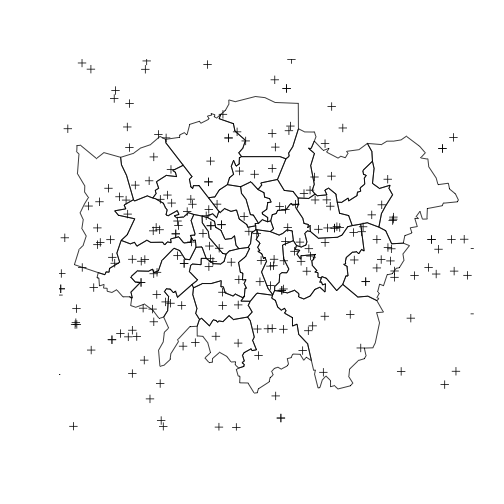
\includegraphics{figure/Input_data_for_a_spatial_join.png}
\caption{Input data for a spatial join}
\end{figure}

The above code reads in a \texttt{SpatialPointsDataFrame} consisting of
2532 transport nodes in and surrounding London and then plots a random
sample of 500 of these over the previously loaded borough level
administrative boundaries. The reason for plotting a sample of the
points rather than all of them is that the boundary data becomes
difficult to see if all of the points are plotted. It is also useful to
see and practice sampling techniques; try to plot only the first 500
points, rather than a random selection, and spot the difference.

The most obvious issue with the point data from the perspective of a
spatial join with the borough data we have is that many of the points in
the dataset are in fact located outside the region of interest. Thus,
the first stage in the analysis is to filter the point data such that
only those that lie within London's administrative zones are selected.
This in itself is a kind of spatial join, and can be accomplished with
the following code.

\begin{Shaded}
\begin{Highlighting}[]
\KeywordTok{proj4string}\NormalTok{(lnd) <- }\KeywordTok{proj4string}\NormalTok{(lnd.stations)}
\NormalTok{lnd.stations <- lnd.stations[lnd, ]  }\CommentTok{# select only points within lnd}
\KeywordTok{plot}\NormalTok{(lnd.stations)  }\CommentTok{# check the result}
\end{Highlighting}
\end{Shaded}
\begin{figure}[htbp]
\centering
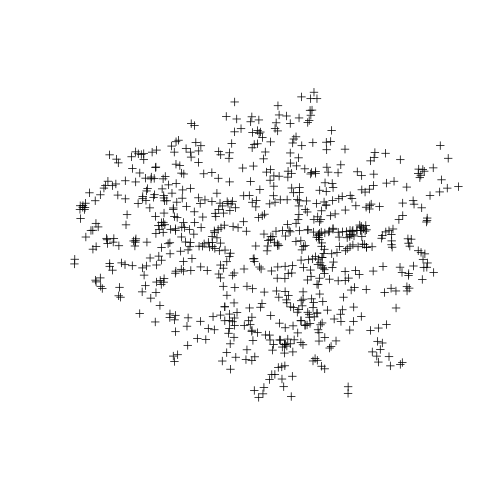
\includegraphics{figure/A_spatial_subset_of_the_points.png}
\caption{A spatial subset of the points}
\end{figure}

The station points now clearly follow the form of the \texttt{lnd}
shape, indicating that the procedure worked. Let's review the code that
allowed this to happen: the first line ensured that the CRS associated
with each layer is \emph{exactly} the same: this step should not be
required in most cases, but it is worth knowing about. Of course, if the
coordinate systems are \emph{actually} different in each layer, the
function \texttt{spTransform} will be needed to make them compatible. In
this case, only the name was slightly different hence direct alteration
of the CRS name via the function \texttt{proj4string}.

The second line of code is where power of R's sp package becomes clear:
all that was needed was to place another spatial object in the row index
of the points (\texttt{{[}lnd, {]}}) and R automatically understood that
a subset based on location should be produced. This line of code is an
example of R's `terseness' - only a single line of code is needed to
perform what is in fact quite a complex operation.

\subsubsection{Spatial aggregation}

Now that only stations which \emph{intersect} with the \texttt{lnd}
polygon have been selected, the next stage is to extract information
about the points within each zone. This many-to-one spatial join is also
known as \emph{spatial aggregation}. To do this there are a couple of
approaches: one using the \texttt{sp} package and the other using
\texttt{rgeos} (see Bivand et al. 2013, 5.3).

As with the \emph{spatial subest} method described above, the developers
of R have been very clever in their implementation of spatial
aggregation methods. To minimise typing and ensure consistency with R's
base functions, \texttt{sp} extends the capabilities of the
\texttt{aggregate} function to automatically detect whether the user is
asking for a spatial or a non-spatial aggregation (they are, in essence,
the same thing - we recommend learning about the non-spatial use of
\texttt{aggregate} in R for comparison).

Continuing with the example of station points in London polygons, let us
use the spatial extension of \texttt{aggregate} to count how many points
are in each borough:

\begin{Shaded}
\begin{Highlighting}[]
\NormalTok{lndStC <- }\KeywordTok{aggregate}\NormalTok{(lnd.stations, }\DataTypeTok{by =} \NormalTok{lnd, }\DataTypeTok{FUN =} \NormalTok{length)}
\KeywordTok{summary}\NormalTok{(lndStC)}
\KeywordTok{plot}\NormalTok{(lndStC)}
\end{Highlighting}
\end{Shaded}
As with the spatial subset function, the above code is extremely terse.
The aggregate function here does three things: 1) identifies which
stations are in which London borough; 2) uses this information to
perform a function on the output, in this case \texttt{length}, which
simply means ``count'' in this context; and 3) creates a new spatial
object equivalent to \texttt{lnd} but with updated attribute data to
reflect the results of the spatial aggregation. The results, with a
legend and colours added, are presented in Figure 9 below. The code used
to create this plot is rather long; it can be viewed online:
http://rpubs.com/RobinLovelace/11738 .

\begin{figure}[htbp]
\centering
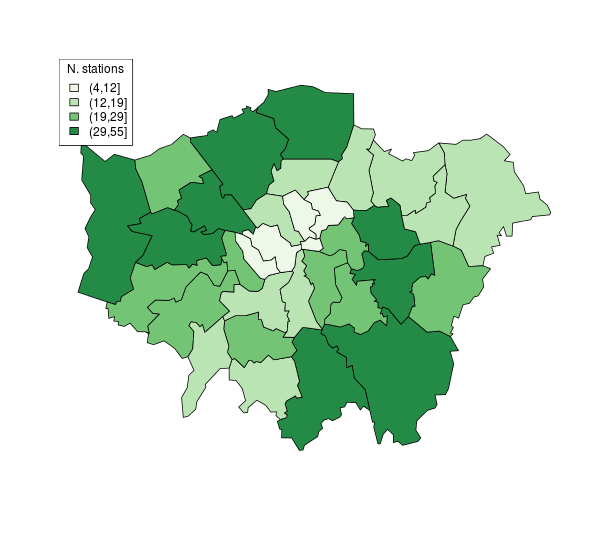
\includegraphics{figure/nStations.png}
\caption{Number of stations in London boroughs}
\end{figure}

As with any spatial attribute data stored as an \texttt{sp} object, we
can look at the attributes of the point data using the \texttt{@}
symbol:

\begin{Shaded}
\begin{Highlighting}[]
\KeywordTok{head}\NormalTok{(lnd.stations@data, }\DataTypeTok{n =} \DecValTok{2}\NormalTok{)}
\end{Highlighting}
\end{Shaded}
\begin{verbatim}
##    CODE          LEGEND FILE_NAME NUMBER                  NAME MICE
## 91 5520 Railway Station  gb_south  17607       Belmont Station   19
## 92 5520 Railway Station  gb_south  17608 Woodmansterne Station    5
\end{verbatim}
In this case we have three potentially interesting variables:
``LEGEND'', telling us what the point is, ``NAME'', and ``MICE'', which
represents the number of mice sightings reported by the public at that
point (this is a fictional variable!). To illustrate the power of the
\texttt{aggregate} function, let us use it to find the average number of
mice spotted in transport points in each London borough, and the
standard deviation:

\begin{Shaded}
\begin{Highlighting}[]
\NormalTok{lndAvMice <- }\KeywordTok{aggregate}\NormalTok{(lnd.stations[}\StringTok{"MICE"}\NormalTok{], }\DataTypeTok{by =} \NormalTok{lnd, }\DataTypeTok{FUN =} \NormalTok{mean)}
\KeywordTok{summary}\NormalTok{(lndAvMice)}
\NormalTok{lndSdMice <- }\KeywordTok{aggregate}\NormalTok{(lnd.stations[}\StringTok{"MICE"}\NormalTok{], }\DataTypeTok{by =} \NormalTok{lnd, }\DataTypeTok{FUN =} \NormalTok{sd)}
\KeywordTok{summary}\NormalTok{(lndSdMice)}
\end{Highlighting}
\end{Shaded}
In the above code, \texttt{aggregate} was used to create entirely new
spatial objects that are exactly the same as \texttt{lnd}, except with
new attribute data. To add the mean mice count to the original object,
the following code can be used:

\begin{Shaded}
\begin{Highlighting}[]
\NormalTok{lnd$av.mice <- lndAvMice$MICE}
\end{Highlighting}
\end{Shaded}
The above code creates a new variable in the \texttt{lnd@data} object
entitled ``av.mice'' and populates it with desired values. Thus
\texttt{Spatial} objects can behave in the same way as data.frames when
refering to attribute variables.

\subsection{Summary}

To summarise this section, we have taken a look inside R's
representation of spatial data, learned how to manipulate these datasets
in terms of CRS transformations and attribute data and finally explored
spatial joins and aggregation.

\section{Fundamentals of Spatial Data Visualisation}

Good maps depend on sound analysis and can have an enormous impact on
the understanding and communication of results. It has never been easier
to produce a map. The underlying data required are available in
unprecedented volumes and the technological capabilities of transforming
them into compelling maps and graphics are increasingly sophisticated
and straightforward to use. Data and software, however, only offer the
starting points of good spatial data visualisation since they need to be
refined and calibrated by the researchers seeking to communicate their
findings. In this section we will run through the features of a good
map. It is worth noting that not all good maps and graphics contain all
the features below -- they should simply be seen as suggestions rather
than firm principles.

Effective map making is hard process -- as Krygier and Wood (2011) put
it ``there is a lot to see, think about, and do''" (p6). It often comes
at the end of a period of intense data analysis and perhaps when the
priority is to get a paper finished or results published and can
therefore be rushed as a result. The beauty of R (and other scripting
languages) is the ability to save code and simply re-run it with
different data. Colours, map adornments and other parameters can
therefore be quickly applied, so it is well worth creating a template
script that adheres to best practice.

We have selected ggplot2 as our package of choice for the bulk of our
maps and spatial data visualisations because it has a number of these
elements at its core. The ``gg''" in its slightly odd name stands for
``Grammar of Graphics''", which is a set of rules developed by Leland
Wilkinson (2005) in a book of the same name. Grammar in the context of
graphics works in much the same way as it does in language - it provides
a structure. The structure is informed by both human perception and also
mathematics to ensure that the resulting visualisations are both
technically sound and comprehensible. By creating ggplot2, Hadley
Wickham, implemented these rules as well as developing ways in which
plots can be built up in layers (see Wickham, 2010). This layering
component is especially useful in the context of spatial data since it
is conceptually the same as map layers in Geographical Information
Systems (GIS).

First ensure that the necessary packages are installed and that R is in
the correct working directory (see above). Then load the packages used
in this section.

\begin{Shaded}
\begin{Highlighting}[]
\KeywordTok{library}\NormalTok{(rgdal)}
\KeywordTok{library}\NormalTok{(ggplot2)}
\KeywordTok{library}\NormalTok{(gridExtra)}
\end{Highlighting}
\end{Shaded}
We are going to use a map of the world to demonstrate some of the
cartographic principles as they are introduced. The world map used is
available from the Natural Earth website. Because these are already
saved in the data folder, we can proceed to load the data.

\begin{Shaded}
\begin{Highlighting}[]
\NormalTok{wrld <- }\KeywordTok{readOGR}\NormalTok{(}\StringTok{"data/"}\NormalTok{, }\StringTok{"ne_110m_admin_0_countries"}\NormalTok{)}
\end{Highlighting}
\end{Shaded}
\begin{verbatim}
## OGR data source with driver: ESRI Shapefile 
## Source: "data/", layer: "ne_110m_admin_0_countries"
## with 177 features and 63 fields
## Feature type: wkbPolygon with 2 dimensions
\end{verbatim}
\begin{Shaded}
\begin{Highlighting}[]
\KeywordTok{plot}\NormalTok{(wrld)}
\end{Highlighting}
\end{Shaded}
\begin{figure}[htbp]
\centering
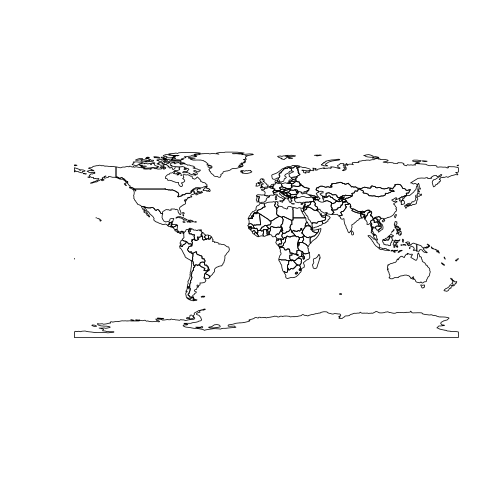
\includegraphics{figure/A_Basic_Map_of_the_World.png}
\caption{A Basic Map of the World}
\end{figure}

Let's see a sample of the attribute data and remove the Falklands and
French Southern and Antarctic Lands (to demonstrate the method - type
\texttt{?regex} if interested how this works - and because these
countries cause continent mis-assignment later on):

\begin{Shaded}
\begin{Highlighting}[]
\KeywordTok{head}\NormalTok{(wrld@data)[}\DecValTok{1}\NormalTok{:}\DecValTok{3}\NormalTok{, }\DecValTok{1}\NormalTok{:}\DecValTok{5}\NormalTok{]}
\end{Highlighting}
\end{Shaded}
\begin{verbatim}
##   scalerank      featurecla labelrank  sovereignt sov_a3
## 0         1 Admin-0 country         3 Afghanistan    AFG
## 1         1 Admin-0 country         3      Angola    AGO
## 2         1 Admin-0 country         6     Albania    ALB
\end{verbatim}
\begin{Shaded}
\begin{Highlighting}[]
\NormalTok{wrld <- wrld[!}\KeywordTok{grepl}\NormalTok{(}\StringTok{"Falk\textbar{}French Southern"}\NormalTok{, wrld$name_long), ]}
\end{Highlighting}
\end{Shaded}
You can see there are a lot of columns associated with this file.
Although we will keep all of them, we are only really interested in the
population estimate (``pop\_est'') field. Before progressing it is is
worth reprojecting the data in order that the population data can be
seen better. The coordinate reference system of the wrld shapefile is
currently WGS84. This is the common latitude and longitude format that
all spatial software packages understand. From a cartographic
perspective the standard plots of this projection, of the kind produced
above, are not suitable since they heavily distort the shapes of those
countries further from the equator. Instead the Robinson projection
provides a good compromise between areal distortion and shape
preservation. We therefore project it as follows.

\begin{Shaded}
\begin{Highlighting}[]
\NormalTok{wrld.rob <- }\KeywordTok{spTransform}\NormalTok{(wrld, }\KeywordTok{CRS}\NormalTok{(}\StringTok{"+proj=robin"}\NormalTok{))}
\KeywordTok{plot}\NormalTok{(wrld.rob)}
\end{Highlighting}
\end{Shaded}
\begin{figure}[htbp]
\centering
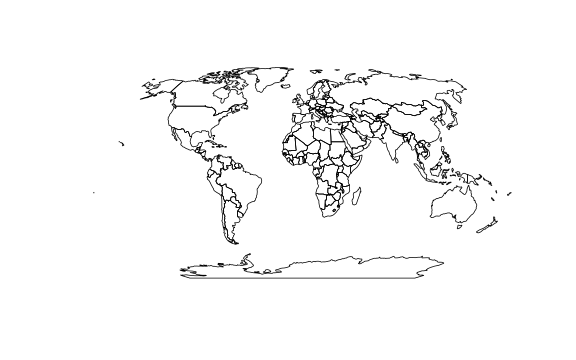
\includegraphics{figure/The_Robinson_Projection.png}
\caption{The Robinson Projection}
\end{figure}

\texttt{+proj=robin} refers to the Robinson prjection. You will have
spotted from the plot that the countries in the world map are much
better proportioned.

We now need to \texttt{fortify} this spatial data to convert it into a
format that ggplot2 understands, we also use \texttt{merge} to re-attach
the attribute data that is lost in the fortify operation.

\begin{Shaded}
\begin{Highlighting}[]
\NormalTok{wrld.rob.f <- }\KeywordTok{fortify}\NormalTok{(wrld.rob, }\DataTypeTok{region =} \StringTok{"sov_a3"}\NormalTok{)}
\end{Highlighting}
\end{Shaded}
\begin{verbatim}
## Loading required package: rgeos
## rgeos version: 0.3-2, (SVN revision 413M)
##  GEOS runtime version: 3.3.8-CAPI-1.7.8 
##  Polygon checking: TRUE
\end{verbatim}
\begin{Shaded}
\begin{Highlighting}[]

\NormalTok{wrld.pop.f <- }\KeywordTok{merge}\NormalTok{(wrld.rob.f, wrld.rob@data, }\DataTypeTok{by.x =} \StringTok{"id"}\NormalTok{, }\DataTypeTok{by.y =} \StringTok{"sov_a3"}\NormalTok{)}
\end{Highlighting}
\end{Shaded}
The code below produces a map coloured by the population variable. It
demonstrates the sophistication of ggplot2 by first stringing together a
series of plot commands and assigning them to a single R object called
\texttt{map}. If you type \texttt{map} into the command line, R will
then execute the code and generate the plot. By simple specifing our
\texttt{fill} variable within the \texttt{aes()} part of the code and
then using the \texttt{geom\_polygon()} command ggplot2 will fill colour
the countries using a default colour pallette and auto-generated key. As
will be shown in the next section these defaults can be easily altered
to produce different looking maps.

\begin{Shaded}
\begin{Highlighting}[]
\NormalTok{map <- }\KeywordTok{ggplot}\NormalTok{(wrld.pop.f, }\KeywordTok{aes}\NormalTok{(long, lat, }\DataTypeTok{group =} \NormalTok{group, }\DataTypeTok{fill =} \NormalTok{pop_est)) + }\KeywordTok{geom_polygon}\NormalTok{() + }
    \KeywordTok{coord_equal}\NormalTok{() + }\KeywordTok{labs}\NormalTok{(}\DataTypeTok{x =} \StringTok{"Longitude"}\NormalTok{, }\DataTypeTok{y =} \StringTok{"Latitude"}\NormalTok{, }\DataTypeTok{fill =} \StringTok{"World Population"}\NormalTok{) + }
    \KeywordTok{ggtitle}\NormalTok{(}\StringTok{"World Population"}\NormalTok{)}

\NormalTok{map}
\end{Highlighting}
\end{Shaded}
\begin{figure}[htbp]
\centering
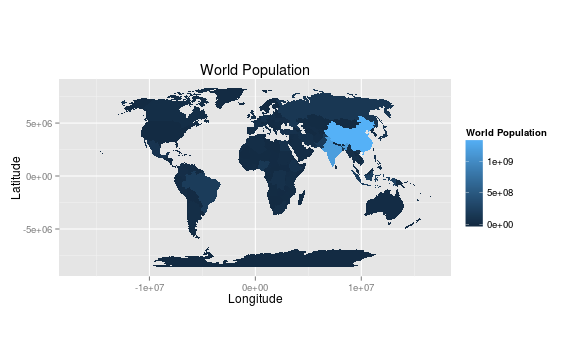
\includegraphics{figure/World_Population_Map.png}
\caption{World Population Map}
\end{figure}

\subsection{Colour and other aesthetics}

Colour has an enormous impact on how people will percieve a graphic.
Readers of a map come to it with a range of pre-conceptions about how
the world looks.

\subsubsection{Choropleth Maps}

ggplot2 knows the different between continuous and categorical (nominal)
data and will automatically assign the appropriate colour palettes when
producing choropleth maps such as the one above. The default colour
palettes are generally a good place to start but users may wish to vary
them for a whole host of reasons, such as the need to print in black and
white. The \texttt{scale\_fill\_} family of commands facilitate such
customisation. For categorical data \texttt{scale\_fill\_manual()} is a
useful command:

\begin{Shaded}
\begin{Highlighting}[]
\CommentTok{# Produce a map of continents}
\NormalTok{map.cont <- }\KeywordTok{ggplot}\NormalTok{(wrld.pop.f, }\KeywordTok{aes}\NormalTok{(long, lat, }\DataTypeTok{group =} \NormalTok{group, }\DataTypeTok{fill =} \NormalTok{continent)) + }
    \KeywordTok{geom_polygon}\NormalTok{() + }\KeywordTok{coord_equal}\NormalTok{() + }\KeywordTok{labs}\NormalTok{(}\DataTypeTok{x =} \StringTok{"Longitude"}\NormalTok{, }\DataTypeTok{y =} \StringTok{"Latitude"}\NormalTok{, }\DataTypeTok{fill =} \StringTok{"World Continents"}\NormalTok{) + }
    \KeywordTok{ggtitle}\NormalTok{(}\StringTok{"World Continents"}\NormalTok{)}

\CommentTok{# To see the default colours}
\NormalTok{map.cont}
\end{Highlighting}
\end{Shaded}
\begin{figure}[htbp]
\centering
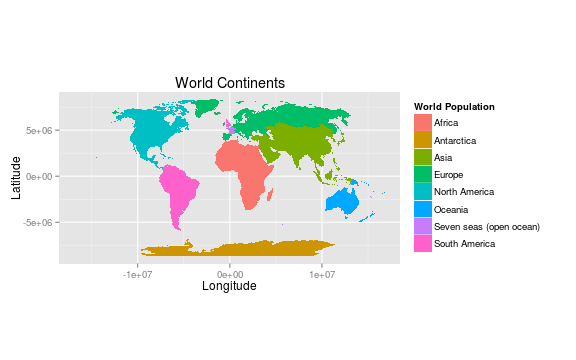
\includegraphics{figure/A_Map_of_the_Continents_Using_Default_Colours.png}
\caption{A Map of the Continents Using Default Colours}
\end{figure}

To change the colour scheme:

\begin{Shaded}
\begin{Highlighting}[]
\NormalTok{map.cont + }\KeywordTok{scale_fill_manual}\NormalTok{(}\DataTypeTok{values =} \KeywordTok{c}\NormalTok{(}\StringTok{"yellow"}\NormalTok{, }\StringTok{"red"}\NormalTok{, }\StringTok{"purple"}\NormalTok{, }\StringTok{"white"}\NormalTok{, }
    \StringTok{"orange"}\NormalTok{, }\StringTok{"blue"}\NormalTok{, }\StringTok{"green"}\NormalTok{, }\StringTok{"black"}\NormalTok{))}
\end{Highlighting}
\end{Shaded}
Whilst \texttt{scale\_fill\_continuous()} works with continuous
datasets:

\begin{Shaded}
\begin{Highlighting}[]
\CommentTok{# note the use of the 'map' object created earler}

\NormalTok{map + }\KeywordTok{scale_fill_continuous}\NormalTok{(}\DataTypeTok{low =} \StringTok{"white"}\NormalTok{, }\DataTypeTok{high =} \StringTok{"black"}\NormalTok{)}
\end{Highlighting}
\end{Shaded}
It is well worth looking at the \emph{Color Brewer} palettes developed
by Cynthia Brewer. These are designed to be colour blind safe and
perceptually uniform such that no one colour jumps out more than any
others. This latter characteristic is important when trying to produce
impartial maps. R has a package that contains the colour palettes and
these can be easily utlised by ggplot2.

\begin{Shaded}
\begin{Highlighting}[]
\KeywordTok{library}\NormalTok{(RColorBrewer)}
\CommentTok{# look at the help documents to see the palettes available. See}
\CommentTok{# http://colorbrewer2.org/}
\StringTok{`}\DataTypeTok{?}\StringTok{`}\NormalTok{(RColorBrewer)}
\CommentTok{# note the use of the scale_fill_gradientn() function rather than}
\CommentTok{# scale_fill_continuous() used above}
\NormalTok{map + }\KeywordTok{scale_fill_gradientn}\NormalTok{(}\DataTypeTok{colours =} \KeywordTok{brewer.pal}\NormalTok{(}\DecValTok{7}\NormalTok{, }\StringTok{"YlGn"}\NormalTok{))}
\end{Highlighting}
\end{Shaded}
In addition to altering the colour scale used to represent continuous
data it may also be desirable to adjust the breaks at which the colour
transitions occur. There are many ways to select both the optimum number
of breaks (i.e colour transtions) and the locations in the dataset at
which they occur. The \texttt{classINT} package contains many ways to
automatically create these breaks. We use the \texttt{grid.arrange}
function from the gridExtra package to display the maps side by side.

\begin{Shaded}
\begin{Highlighting}[]
\KeywordTok{library}\NormalTok{(classInt)}

\CommentTok{# Specify how many breaks you want - generally this should be fewer than 7.}

\NormalTok{nbrks <- }\DecValTok{6}

\CommentTok{# Here quantiles are used to identify the breaks (note that we are using the}
\CommentTok{# original 'wrld.rob' object and not the 'wrld.rob@data$pop_est.f'). USe the}
\CommentTok{# help files to see the full range of options.}
\NormalTok{brks <- }\KeywordTok{classIntervals}\NormalTok{(wrld.rob@data$pop_est, }\DataTypeTok{n =} \NormalTok{nbrks, }\DataTypeTok{style =} \StringTok{"quantile"}\NormalTok{)}

\KeywordTok{print}\NormalTok{(brks)}
\end{Highlighting}
\end{Shaded}
\begin{verbatim}
## style: quantile
##        [-99,1990876)    [1990876,4615807)    [4615807,9059651) 
##                   29                   29                   29 
##   [9059651,16715999)  [16715999,40913584) [40913584,1.339e+09] 
##                   29                   29                   30
\end{verbatim}
\begin{Shaded}
\begin{Highlighting}[]

\CommentTok{# Now the breaks can be easily inserted into the code above for a range of}
\CommentTok{# colour palettes}
\NormalTok{YlGn <- map + }\KeywordTok{scale_fill_gradientn}\NormalTok{(}\DataTypeTok{colours =} \KeywordTok{brewer.pal}\NormalTok{(nbrks, }\StringTok{"YlGn"}\NormalTok{), }\DataTypeTok{breaks =} \KeywordTok{c}\NormalTok{(brks$brks))}

\NormalTok{PuBu <- map + }\KeywordTok{scale_fill_gradientn}\NormalTok{(}\DataTypeTok{colours =} \KeywordTok{brewer.pal}\NormalTok{(nbrks, }\StringTok{"PuBu"}\NormalTok{), }\DataTypeTok{breaks =} \KeywordTok{c}\NormalTok{(brks$brks))}

\KeywordTok{grid.arrange}\NormalTok{(YlGn, PuBu, }\DataTypeTok{ncol =} \DecValTok{2}\NormalTok{)}
\end{Highlighting}
\end{Shaded}
If you are not happy with the automatic methods of specifying breaks it
can also be done manually:

\begin{Shaded}
\begin{Highlighting}[]
\KeywordTok{library}\NormalTok{()}
\NormalTok{nbrks <- }\DecValTok{4}
\NormalTok{brks <- }\KeywordTok{c}\NormalTok{(}\FloatTok{1e+08}\NormalTok{, }\FloatTok{2.5e+08}\NormalTok{, }\FloatTok{5e+07}\NormalTok{, }\FloatTok{1e+09}\NormalTok{)}
\NormalTok{map + }\KeywordTok{scale_fill_gradientn}\NormalTok{(}\DataTypeTok{colours =} \KeywordTok{brewer.pal}\NormalTok{(nbrks, }\StringTok{"PuBu"}\NormalTok{), }\DataTypeTok{breaks =} \KeywordTok{c}\NormalTok{(brks))}
\end{Highlighting}
\end{Shaded}
\begin{figure}[htbp]
\centering
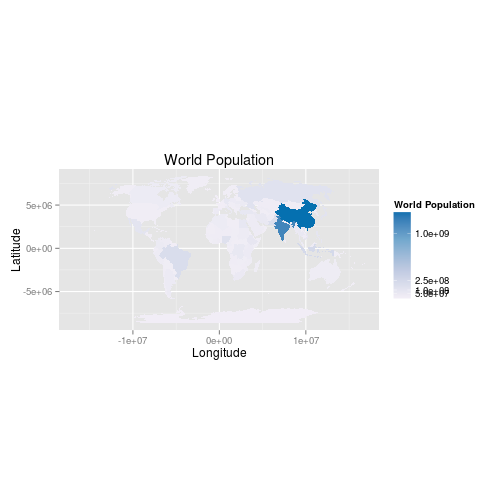
\includegraphics{figure/unnamed-chunk-5.png}
\caption{unnamed-chunk-5}
\end{figure}

There are many other ways to specify and alter the colours in ggplot2
and these are outlined in the help documentation. There are also many
examples online.

If the map's purpose is to clearly communicate data then it is often
advisable to conform to conventions so as not to disorientate readers to
ensure they can focus on the key messages contained in the data. A good
example of this is the use of blue for bodies of water and green for
landmasses. The code example below generates two plots with our
wrld.pop.f object. The first colours the land blue and the sea (in this
case the background to the map) green and the second is more
conventional.

\begin{Shaded}
\begin{Highlighting}[]
\NormalTok{map2 <- }\KeywordTok{ggplot}\NormalTok{(wrld.pop.f, }\KeywordTok{aes}\NormalTok{(long, lat, }\DataTypeTok{group =} \NormalTok{group)) + }\KeywordTok{coord_equal}\NormalTok{()}

\NormalTok{blue <- map2 + }\KeywordTok{geom_polygon}\NormalTok{(}\DataTypeTok{fill =} \StringTok{"light blue"}\NormalTok{) + }\KeywordTok{theme}\NormalTok{(}\DataTypeTok{panel.background =} \KeywordTok{element_rect}\NormalTok{(}\DataTypeTok{fill =} \StringTok{"dark green"}\NormalTok{))}

\NormalTok{green <- map2 + }\KeywordTok{geom_polygon}\NormalTok{(}\DataTypeTok{fill =} \StringTok{"dark green"}\NormalTok{) + }\KeywordTok{theme}\NormalTok{(}\DataTypeTok{panel.background =} \KeywordTok{element_rect}\NormalTok{(}\DataTypeTok{fill =} \StringTok{"light blue"}\NormalTok{))}

\KeywordTok{grid.arrange}\NormalTok{(blue, green, }\DataTypeTok{ncol =} \DecValTok{2}\NormalTok{)}
\end{Highlighting}
\end{Shaded}
\begin{figure}[htbp]
\centering
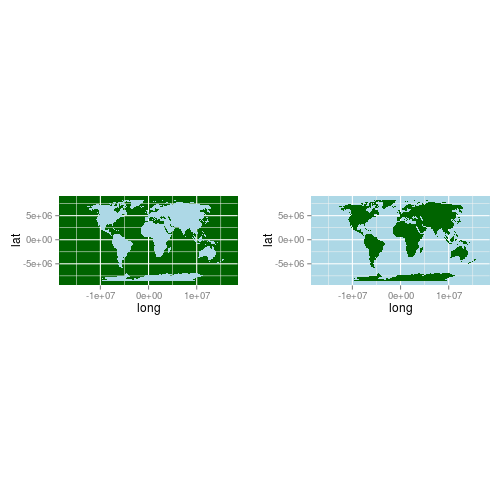
\includegraphics{figure/Conforming_to_Colour_Convention.png}
\caption{Conforming to Colour Convention}
\end{figure}

\subsubsection{Experimenting with line colour and line widths}

In addition to conforming to colour conventions, line colour and width
offer important parameters, which are often overlooked tools for
increasing the legibility of a graphic. As the code below demonstrates,
it is possible to adjust line colour through using the \texttt{colour}
parameter and the line width using the \texttt{lwd} parameter. The
impact of different line widths will vary depending on your screen size
and resolution. If you save the plot to pdf (or an image) then the size
at which you do this will also affect the line widths.

\begin{Shaded}
\begin{Highlighting}[]
\NormalTok{map3 <- map2 + }\KeywordTok{theme}\NormalTok{(}\DataTypeTok{panel.background =} \KeywordTok{element_rect}\NormalTok{(}\DataTypeTok{fill =} \StringTok{"light blue"}\NormalTok{))}

\NormalTok{yellow <- map3 + }\KeywordTok{geom_polygon}\NormalTok{(}\DataTypeTok{fill =} \StringTok{"dark green"}\NormalTok{, }\DataTypeTok{colour =} \StringTok{"yellow"}\NormalTok{)}

\NormalTok{black <- map3 + }\KeywordTok{geom_polygon}\NormalTok{(}\DataTypeTok{fill =} \StringTok{"dark green"}\NormalTok{, }\DataTypeTok{colour =} \StringTok{"black"}\NormalTok{)}

\NormalTok{thin <- map3 + }\KeywordTok{geom_polygon}\NormalTok{(}\DataTypeTok{fill =} \StringTok{"dark green"}\NormalTok{, }\DataTypeTok{colour =} \StringTok{"black"}\NormalTok{, }\DataTypeTok{lwd =} \FloatTok{0.1}\NormalTok{)}

\NormalTok{thick <- map3 + }\KeywordTok{geom_polygon}\NormalTok{(}\DataTypeTok{fill =} \StringTok{"dark green"}\NormalTok{, }\DataTypeTok{colour =} \StringTok{"black"}\NormalTok{, }\DataTypeTok{lwd =} \FloatTok{1.5}\NormalTok{)}

\KeywordTok{grid.arrange}\NormalTok{(yellow, black, thick, thin, }\DataTypeTok{ncol =} \DecValTok{2}\NormalTok{)}
\end{Highlighting}
\end{Shaded}
\begin{figure}[htbp]
\centering
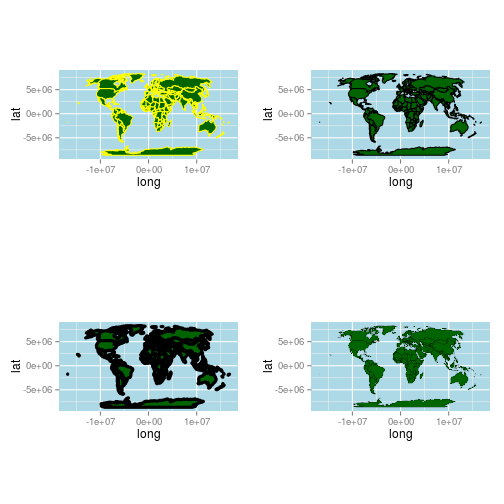
\includegraphics{figure/The_Impact_of_Line_Width.png}
\caption{The Impact of Line Width}
\end{figure}

There are other parameters such as layer transparency (use the
\texttt{alpha} parameter for this) that can be applied to all aspects of
the plot - both points, lines and polygons. Space does not permit their
full exploration here but more information is available from the many
online examples and the ggplot2 package documentation.

\subsection{Map Adornments and Annotations}

Map adornments and annotations are essential to orientate the viewer and
provide context; they include graticules, north arrows, scale bars and
data attribution. Not all are required on a single map, indeed it is
often best that they are used sparingly to avoid unecessary clutter
(Monkhouse and Wilkinson, 1971). With ggplot2 many of these are added
automatically but they can be customised.

\subsubsection{North arrow}

In the maps created so far, we have defined the \emph{aesthetics} of the
map in the foundation function ggplot. The result of this is that all
subsequent layers are expected to have the same variables and
essentially contain data with the same dimensions as original dataset.
But what if we want to add a new layer from a completely different
dataset, e.g.~to add an arrow? To do this, we must not add any arguments
to the \texttt{ggplot} function, only adding data sources one layer at a
time:

Here we create an empty plot, meaning that each new layer must be given
its own dataset. While more code is needed in this example, it enables
much greater flexibility with regards to what can be included in new
layer contents. Another possibility is to use \texttt{geom\_segment()}
to add a rudimentary arrow (see \texttt{?geom\_segment} for
refinements):

\begin{Shaded}
\begin{Highlighting}[]
\KeywordTok{library}\NormalTok{(grid)  }\CommentTok{# needed for arrow}
\KeywordTok{ggplot}\NormalTok{() + }\KeywordTok{geom_polygon}\NormalTok{(}\DataTypeTok{data =} \NormalTok{wrld.pop.f, }\KeywordTok{aes}\NormalTok{(long, lat, }\DataTypeTok{group =} \NormalTok{group, }\DataTypeTok{fill =} \NormalTok{pop_est)) + }
    \KeywordTok{geom_line}\NormalTok{(}\KeywordTok{aes}\NormalTok{(}\DataTypeTok{x =} \KeywordTok{c}\NormalTok{(-}\FloatTok{1.3e+07}\NormalTok{, -}\FloatTok{1.3e+07}\NormalTok{), }\DataTypeTok{y =} \KeywordTok{c}\NormalTok{(}\DecValTok{0}\NormalTok{, }\FloatTok{5e+06}\NormalTok{)), }\DataTypeTok{arrow =} \KeywordTok{arrow}\NormalTok{()) + }
    \KeywordTok{coord_fixed}\NormalTok{()  }\CommentTok{# correct aspect ratio}
\end{Highlighting}
\end{Shaded}
\begin{figure}[htbp]
\centering
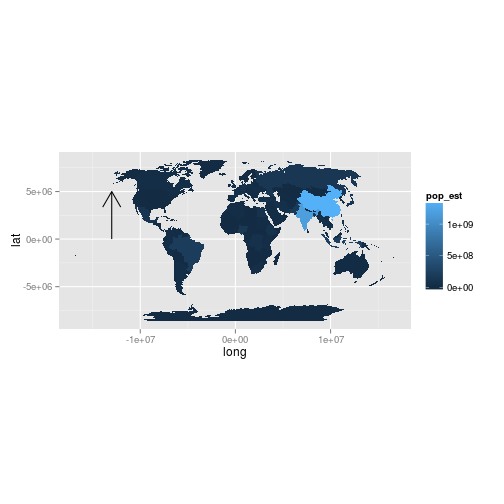
\includegraphics{figure/North_Arrow_Example.png}
\caption{North Arrow Example}
\end{figure}

\subsubsection{Scale bar}

ggplot2's scale bar capabilities are perhaps the least satisfactory
element of the package. For this example we use the
\texttt{geom\_line()} function to draw a line of approximately 1km in
length using the \texttt{lnd.f} object containing the London Boroughs
discussed in Section 2. The reason for this is that it is in a projected
coordinate system - British National Grid - so each map unit is worth
1m. In the case of the world map the distances at the equator in terms
of degrees east to west are very different from those further north or
south. Any line drawn using the the simple approach below would
therefore be inaccurate. For maps covering large areas - such as the
entire world - leaving the axis labels on will enable them to act as a
graticule which will indicate distance.

\begin{Shaded}
\begin{Highlighting}[]
\KeywordTok{load}\NormalTok{(}\StringTok{"data/lnd.f.RData"}\NormalTok{)}
\KeywordTok{ggplot}\NormalTok{() + }\KeywordTok{geom_polygon}\NormalTok{(}\DataTypeTok{data =} \NormalTok{lnd.f, }\KeywordTok{aes}\NormalTok{(long, lat, }\DataTypeTok{group =} \NormalTok{group)) + }\KeywordTok{geom_line}\NormalTok{(}\KeywordTok{aes}\NormalTok{(}\DataTypeTok{x =} \KeywordTok{c}\NormalTok{(}\DecValTok{505000}\NormalTok{, }
    \DecValTok{515000}\NormalTok{), }\DataTypeTok{y =} \KeywordTok{c}\NormalTok{(}\DecValTok{158000}\NormalTok{, }\DecValTok{158000}\NormalTok{)), }\DataTypeTok{lwd =} \DecValTok{2}\NormalTok{) + }\KeywordTok{annotate}\NormalTok{(}\StringTok{"text"}\NormalTok{, }\DataTypeTok{label =} \StringTok{"10km"}\NormalTok{, }
    \DataTypeTok{x =} \DecValTok{510000}\NormalTok{, }\DataTypeTok{y =} \DecValTok{160000}\NormalTok{) + }\KeywordTok{coord_fixed}\NormalTok{()}
\end{Highlighting}
\end{Shaded}
\begin{figure}[htbp]
\centering
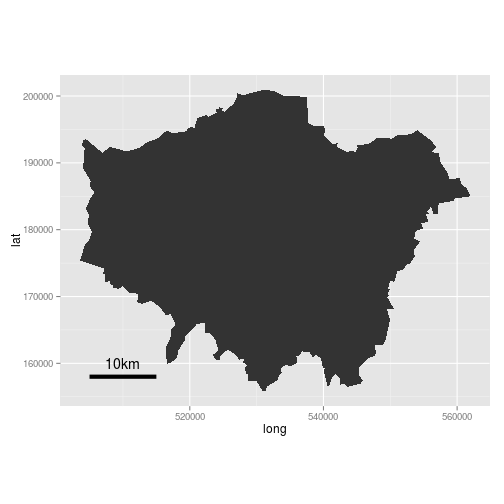
\includegraphics{figure/Scale_Bar_Example.png}
\caption{Scale Bar Example}
\end{figure}

\subsubsection{Legends}

Legends are added automatically but can be customised in a number of
ways. A few examples are included below with more details avaialble in
the \texttt{ggplot2} documentation.

\begin{Shaded}
\begin{Highlighting}[]
\CommentTok{# Position}
\NormalTok{map + }\KeywordTok{theme}\NormalTok{(}\DataTypeTok{legend.position =} \StringTok{"top"}\NormalTok{)}
\end{Highlighting}
\end{Shaded}
\begin{figure}[htbp]
\centering
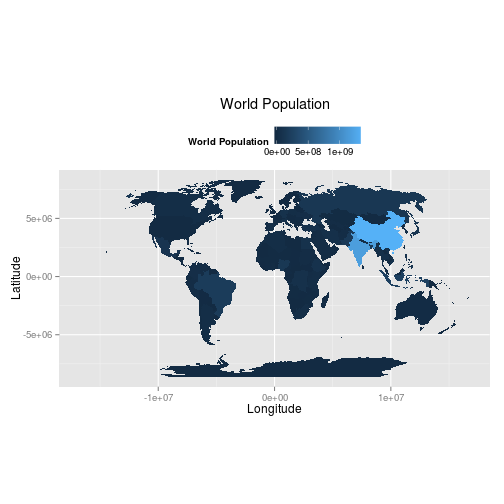
\includegraphics{figure/Formatting_the_Legend.png}
\caption{Formatting the Legend}
\end{figure}

As you can see, this added the legend in a new place. Many more options
for customization are available, as highlighed in the examples below.

\begin{Shaded}
\begin{Highlighting}[]
\CommentTok{# Title}
\NormalTok{map + }\KeywordTok{theme}\NormalTok{(}\DataTypeTok{legend.title =} \KeywordTok{element_text}\NormalTok{(}\DataTypeTok{colour =} \StringTok{"Red"}\NormalTok{, }\DataTypeTok{size =} \DecValTok{16}\NormalTok{, }\DataTypeTok{face =} \StringTok{"bold"}\NormalTok{))}

\CommentTok{# Label Font Size and Colour}
\NormalTok{map + }\KeywordTok{theme}\NormalTok{(}\DataTypeTok{legend.text =} \KeywordTok{element_text}\NormalTok{(}\DataTypeTok{colour =} \StringTok{"blue"}\NormalTok{, }\DataTypeTok{size =} \DecValTok{16}\NormalTok{, }\DataTypeTok{face =} \StringTok{"italic"}\NormalTok{))}

\CommentTok{# Border and background box}
\NormalTok{map + }\KeywordTok{theme}\NormalTok{(}\DataTypeTok{legend.background =} \KeywordTok{element_rect}\NormalTok{(}\DataTypeTok{fill =} \StringTok{"gray90"}\NormalTok{, }\DataTypeTok{size =} \FloatTok{0.5}\NormalTok{, }\DataTypeTok{linetype =} \StringTok{"dotted"}\NormalTok{))}
\end{Highlighting}
\end{Shaded}
\subsection{Adding Basemaps To Your Plots}

The development of the ggmap package has enabled the simple use of
online mapping services such as Google Maps and OpenStreetMap for base
maps. Using image tiles from these services spatial data can be placed
in context as users can easily orientate themselves to streets and
landmarks.

For this example we are going to use the shapefile of London sports
participation introduced in Section 2. The data were originally
projected to British National Grid (BNG) which is not compatible with
the online map services used in the following examples. It therefore
needs reprojecting - a step we completed earlier. The reprojected file
can be loaded as follows:

\begin{Shaded}
\begin{Highlighting}[]
\KeywordTok{load}\NormalTok{(}\StringTok{"data/lnd.wgs84.RData"}\NormalTok{)}
\end{Highlighting}
\end{Shaded}
The first job is to calculate the bounding box (bb for short) of the
\texttt{lnd.wgs84} object to identify the geographic extent of the map.
This information is used to request the appropriate map tiles from the
map service of our choice. This process is conceptually the same as the
size of your web browser or smartphone screen when using Google maps for
navigation. The first line of code in the snippet below retrieves the
bounding box and the two that follow add 5\% so there is a little space
around the edges of the data to be plotted.

\begin{Shaded}
\begin{Highlighting}[]
\NormalTok{b <- }\KeywordTok{bbox}\NormalTok{(lnd.wgs84)}
\NormalTok{b[}\DecValTok{1}\NormalTok{, ] <- (b[}\DecValTok{1}\NormalTok{, ] - }\KeywordTok{mean}\NormalTok{(b[}\DecValTok{1}\NormalTok{, ])) * }\FloatTok{1.05} \NormalTok{+ }\KeywordTok{mean}\NormalTok{(b[}\DecValTok{1}\NormalTok{, ])}
\NormalTok{b[}\DecValTok{2}\NormalTok{, ] <- (b[}\DecValTok{2}\NormalTok{, ] - }\KeywordTok{mean}\NormalTok{(b[}\DecValTok{2}\NormalTok{, ])) * }\FloatTok{1.05} \NormalTok{+ }\KeywordTok{mean}\NormalTok{(b[}\DecValTok{2}\NormalTok{, ])}
\CommentTok{# scale longitude and latitude (increase bb by 5% for plot) replace 1.05}
\CommentTok{# with 1.xx for an xx% increase in the plot size}
\end{Highlighting}
\end{Shaded}
This is then fed into the \texttt{get\_map} function as the location
parameter. The syntax below contains 2 functions. \texttt{ggmap} is
required to produce the plot and provides the base map data.

\begin{Shaded}
\begin{Highlighting}[]
\KeywordTok{library}\NormalTok{(ggmap)}

\NormalTok{lnd.b1 <- }\KeywordTok{ggmap}\NormalTok{(}\KeywordTok{get_map}\NormalTok{(}\DataTypeTok{location =} \NormalTok{b))}
\end{Highlighting}
\end{Shaded}
\begin{verbatim}
## Warning: bounding box given to google - spatial extent only approximate.
\end{verbatim}
\texttt{ggmap} follows the same syntax structures as ggplot2 and so can
easily be integrated with the other examples included here. First
\texttt{fortify} the \texttt{lnd.wgs84} object and then merge with the
required attribute data.

\begin{Shaded}
\begin{Highlighting}[]
\NormalTok{lnd.wgs84.f <- }\KeywordTok{fortify}\NormalTok{(lnd.wgs84, }\DataTypeTok{region =} \StringTok{"ons_label"}\NormalTok{)}
\NormalTok{lnd.wgs84.f <- }\KeywordTok{merge}\NormalTok{(lnd.wgs84.f, lnd.wgs84@data, }\DataTypeTok{by.x =} \StringTok{"id"}\NormalTok{, }\DataTypeTok{by.y =} \StringTok{"ons_label"}\NormalTok{)}
\end{Highlighting}
\end{Shaded}
We can now overlay this on our base map using the
\texttt{geom\_polygon()} function.

\begin{Shaded}
\begin{Highlighting}[]
\NormalTok{lnd.b1 + }\KeywordTok{geom_polygon}\NormalTok{(}\DataTypeTok{data =} \NormalTok{lnd.wgs84.f, }\KeywordTok{aes}\NormalTok{(}\DataTypeTok{x =} \NormalTok{long, }\DataTypeTok{y =} \NormalTok{lat, }\DataTypeTok{group =} \NormalTok{group, }
    \DataTypeTok{fill =} \NormalTok{Partic_Per), }\DataTypeTok{alpha =} \FloatTok{0.5}\NormalTok{)}
\end{Highlighting}
\end{Shaded}
The resulting map looks reasonable, but it would be improved with a
simpler base map in black and white. A design firm called \emph{stamen}
provide the tiles we need and they can be brought into the plot with the
\texttt{get\_map} function:

\begin{Shaded}
\begin{Highlighting}[]
\NormalTok{lnd.b2 <- }\KeywordTok{ggmap}\NormalTok{(}\KeywordTok{get_map}\NormalTok{(}\DataTypeTok{location =} \NormalTok{b, }\DataTypeTok{source =} \StringTok{"stamen"}\NormalTok{, }\DataTypeTok{maptype =} \StringTok{"toner"}\NormalTok{, }
    \DataTypeTok{crop =} \NormalTok{T))  }\CommentTok{#note the addition of the maptype parameter.}
\end{Highlighting}
\end{Shaded}
We can then produce the plot as before.

\begin{Shaded}
\begin{Highlighting}[]
\NormalTok{lnd.b2 + }\KeywordTok{geom_polygon}\NormalTok{(}\DataTypeTok{data =} \NormalTok{lnd.wgs84.f, }\KeywordTok{aes}\NormalTok{(}\DataTypeTok{x =} \NormalTok{long, }\DataTypeTok{y =} \NormalTok{lat, }\DataTypeTok{group =} \NormalTok{group, }
    \DataTypeTok{fill =} \NormalTok{Partic_Per), }\DataTypeTok{alpha =} \FloatTok{0.5}\NormalTok{)}
\end{Highlighting}
\end{Shaded}
Finally, if we want to increase the detail of the base map,
\texttt{get\_map} has a zoom parameter.

\begin{Shaded}
\begin{Highlighting}[]
\NormalTok{lnd.b3 <- }\KeywordTok{ggmap}\NormalTok{(}\KeywordTok{get_map}\NormalTok{(}\DataTypeTok{location =} \NormalTok{b, }\DataTypeTok{source =} \StringTok{"stamen"}\NormalTok{, }\DataTypeTok{maptype =} \StringTok{"toner"}\NormalTok{, }
    \DataTypeTok{crop =} \NormalTok{T, }\DataTypeTok{zoom =} \DecValTok{11}\NormalTok{))}

\NormalTok{lnd.b3 + }\KeywordTok{geom_polygon}\NormalTok{(}\DataTypeTok{data =} \NormalTok{lnd.wgs84.f, }\KeywordTok{aes}\NormalTok{(}\DataTypeTok{x =} \NormalTok{long, }\DataTypeTok{y =} \NormalTok{lat, }\DataTypeTok{group =} \NormalTok{group, }
    \DataTypeTok{fill =} \NormalTok{Partic_Per), }\DataTypeTok{alpha =} \FloatTok{0.5}\NormalTok{)}
\end{Highlighting}
\end{Shaded}
\begin{figure}[htbp]
\centering
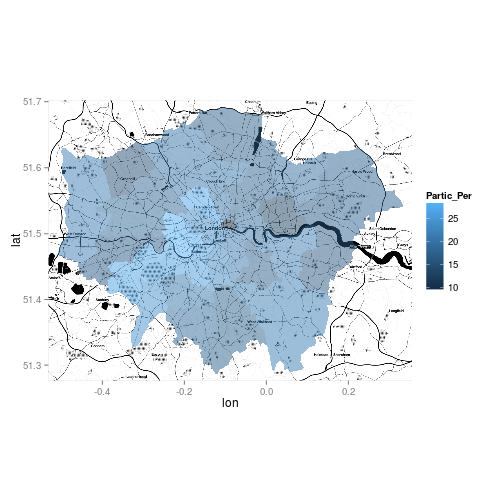
\includegraphics{figure/Using_the_Stamen_Toner_basemap.png}
\caption{Using the Stamen Toner basemap}
\end{figure}

Spatial polygons are not the only data types compatible with
\texttt{ggmap} - you can use any plot type and set of parameters
available in \texttt{ggplot2}, making it an ideal companion package for
spatial data visualisation.

\subsection{Summary}

There are an almost infinite number of different combinations colours,
adornments and line widths that could be applied to a map, so take
inspiration from maps and graphics you have seen and liked. The process
is an iterative one, it will take multiple attempts to get right. Show
your map to friends and colleagues - all will have an opinion but don't
be afraid to stand by the decisions you have taken. To give your maps a
final polish you may wish to export them as a pdf using the
\texttt{ggsave()} function and importing them into a vector graphics
package such as Adobe Illustrator or Inkscape.

The beauty of producing maps in a programming environment as opposed to
the GUI offered by the majority of GIS software packages lies in the
fact that each line of code can be easily adapted to a different
dataset. Users can therefore create a series of scripts that act as
templates and simply call them when required. This saves a huge amount
of time and has the added advantage that all outputs will have a
consistent style and thus offer more professional looking publications.

\section{A Final Example}

Here we present a final example that draws upon the many advanced
concepts discussed in this tutorial to produce a map of 18th Century
Shipping flows. The data have been obtained from the CLIWOC project and
they represent a sample of digitised ships' logs from the 18th Century.
We are using a very small sample of the the full dataset, which is
available from here: http://pendientedemigracion.ucm.es/info/cliwoc/.
The example has been chosen to demonstrate a range of capabilities
within ggplot2 and the ways in which they can be applied to produce
high-quality maps with only a few lines of code. We end by showing how
the maps can be animated to chart the routes over time and the ability
of R to produce many maps very quickly.

As always, the first step is to load in the required packages and
datasets. Here we are using the png package to load in a series of map
annotations. These have been created in image editing software and will
add a historic feel to the map. We are also loading in a World boundary
shapefile and the shipping data itself.

\begin{Shaded}
\begin{Highlighting}[]
\KeywordTok{library}\NormalTok{(rgdal)}
\KeywordTok{library}\NormalTok{(ggplot2)}
\KeywordTok{library}\NormalTok{(png)}
\NormalTok{wrld <- }\KeywordTok{readOGR}\NormalTok{(}\StringTok{"data/"}\NormalTok{, }\StringTok{"ne_110m_admin_0_countries"}\NormalTok{)}
\end{Highlighting}
\end{Shaded}
\begin{verbatim}
## OGR data source with driver: ESRI Shapefile 
## Source: "data/", layer: "ne_110m_admin_0_countries"
## with 177 features and 63 fields
## Feature type: wkbPolygon with 2 dimensions
\end{verbatim}
\begin{Shaded}
\begin{Highlighting}[]
\NormalTok{btitle <- }\KeywordTok{readPNG}\NormalTok{(}\StringTok{"figure/brit_titles.png"}\NormalTok{)}
\NormalTok{compass <- }\KeywordTok{readPNG}\NormalTok{(}\StringTok{"figure/windrose.png"}\NormalTok{)}
\NormalTok{bdata <- }\KeywordTok{read.csv}\NormalTok{(}\StringTok{"data/british_shipping_example.csv"}\NormalTok{)}
\end{Highlighting}
\end{Shaded}
If you look at the first few lines in the \texttt{bdata} object you will
see there are 7 columns with each row representing a single point on the
ships course. The year of the journey and the nationality of the ship
are also included. The final 3 columns are identifiers that are used
later to group the coordinate points together into the paths that
ggplot2 plots.

We first specify some plot parameters that remove the axis labels.

\begin{Shaded}
\begin{Highlighting}[]
\NormalTok{xquiet <- }\KeywordTok{scale_x_continuous}\NormalTok{(}\StringTok{""}\NormalTok{, }\DataTypeTok{breaks =} \OtherTok{NULL}\NormalTok{)}
\NormalTok{yquiet <- }\KeywordTok{scale_y_continuous}\NormalTok{(}\StringTok{""}\NormalTok{, }\DataTypeTok{breaks =} \OtherTok{NULL}\NormalTok{)}
\NormalTok{quiet <- }\KeywordTok{list}\NormalTok{(xquiet, yquiet)}
\end{Highlighting}
\end{Shaded}
The next step is to \texttt{fortify} the World coastlines and create the
base plot. This sets the extents of the plot window and provides the
blank canvas on which we will build up the layers. The first layer
created is the wrld object; the code is wrapped in \texttt{c()} to
prevent it from executing by simply storing it as the plot's parameters.

\begin{Shaded}
\begin{Highlighting}[]
\NormalTok{wrld.f <- }\KeywordTok{fortify}\NormalTok{(wrld, }\DataTypeTok{region =} \StringTok{"sov_a3"}\NormalTok{)}
\end{Highlighting}
\end{Shaded}
\begin{verbatim}
## Loading required package: rgeos
## rgeos version: 0.3-2, (SVN revision 413M)
##  GEOS runtime version: 3.3.8-CAPI-1.7.8 
##  Polygon checking: TRUE
\end{verbatim}
\begin{Shaded}
\begin{Highlighting}[]
\NormalTok{base <- }\KeywordTok{ggplot}\NormalTok{(wrld.f, }\KeywordTok{aes}\NormalTok{(}\DataTypeTok{x =} \NormalTok{long, }\DataTypeTok{y =} \NormalTok{lat))}
\NormalTok{wrld <- }\KeywordTok{c}\NormalTok{(}\KeywordTok{geom_polygon}\NormalTok{(}\KeywordTok{aes}\NormalTok{(}\DataTypeTok{group =} \NormalTok{group), }\DataTypeTok{size =} \FloatTok{0.1}\NormalTok{, }\DataTypeTok{colour =} \StringTok{"black"}\NormalTok{, }\DataTypeTok{fill =} \StringTok{"#D6BF86"}\NormalTok{, }
    \DataTypeTok{data =} \NormalTok{wrld.f, }\DataTypeTok{alpha =} \DecValTok{1}\NormalTok{))}
\end{Highlighting}
\end{Shaded}
To see the result of this simply type:

\begin{Shaded}
\begin{Highlighting}[]
\NormalTok{base + wrld}
\end{Highlighting}
\end{Shaded}
\begin{figure}[htbp]
\centering
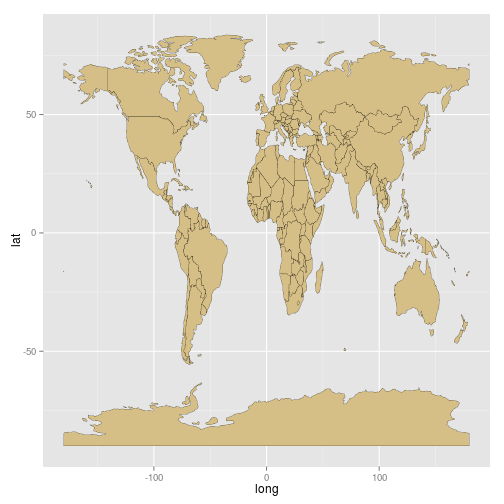
\includegraphics{figure/World_Map.png}
\caption{World Map}
\end{figure}

The code snipped below creates the plot layer containing the the
shipping routes. The \texttt{geom\_path()} function is used to string
together the coordinates into the routes. You can see within the
\texttt{aes()} component we have specified long and lat plus pasted
together the trp and \texttt{group.regroup} variables to identify the
unique paths.

\begin{Shaded}
\begin{Highlighting}[]
\NormalTok{route <- }\KeywordTok{c}\NormalTok{(}\KeywordTok{geom_path}\NormalTok{(}\KeywordTok{aes}\NormalTok{(long, lat, }\DataTypeTok{group =} \KeywordTok{paste}\NormalTok{(bdata$trp, bdata$group.regroup, }
    \DataTypeTok{sep =} \StringTok{"."}\NormalTok{)), }\DataTypeTok{colour =} \StringTok{"#0F3B5F"}\NormalTok{, }\DataTypeTok{size =} \FloatTok{0.2}\NormalTok{, }\DataTypeTok{data =} \NormalTok{bdata, }\DataTypeTok{alpha =} \FloatTok{0.5}\NormalTok{, }
    \DataTypeTok{lineend =} \StringTok{"round"}\NormalTok{))}
\end{Highlighting}
\end{Shaded}
We now have all we need to generate the final plot by building the
layers together with the \texttt{+} sign as shown in the code below. The
first 3 arguments are the plot layers, and the parameters within
\texttt{theme()} are changing the background colour to sea blue.
\texttt{annotation\_raster()} plots the png map adornments loaded in
earlier- this requires the bounding box of each image to be specified.
In this case we use latitude and longitude (in WGS84) and we can use
these paramrters to change the png's position and also its size. The
final two arguments fix the aspect ratio of the plot and remove the axis
labels.

\begin{Shaded}
\begin{Highlighting}[]
\NormalTok{base + route + wrld + }\KeywordTok{theme}\NormalTok{(}\DataTypeTok{panel.background =} \KeywordTok{element_rect}\NormalTok{(}\DataTypeTok{fill =} \StringTok{"#BAC4B9"}\NormalTok{, }
    \DataTypeTok{colour =} \StringTok{"black"}\NormalTok{)) + }\KeywordTok{annotation_raster}\NormalTok{(btitle, }\DataTypeTok{xmin =} \DecValTok{30}\NormalTok{, }\DataTypeTok{xmax =} \DecValTok{140}\NormalTok{, }\DataTypeTok{ymin =} \DecValTok{51}\NormalTok{, }
    \DataTypeTok{ymax =} \DecValTok{87}\NormalTok{) + }\KeywordTok{annotation_raster}\NormalTok{(compass, }\DataTypeTok{xmin =} \DecValTok{65}\NormalTok{, }\DataTypeTok{xmax =} \DecValTok{105}\NormalTok{, }\DataTypeTok{ymin =} \DecValTok{25}\NormalTok{, }
    \DataTypeTok{ymax =} \DecValTok{65}\NormalTok{) + }\KeywordTok{coord_equal}\NormalTok{() + quiet}
\end{Highlighting}
\end{Shaded}
\begin{figure}[htbp]
\centering
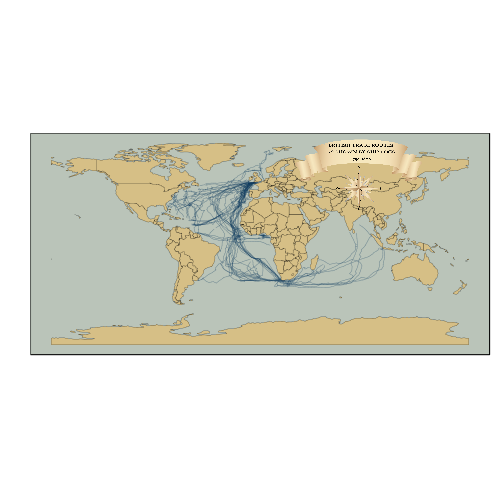
\includegraphics{figure/World_Shipping.png}
\caption{World Shipping}
\end{figure}

In the plot example we have chosen the colours carefully to give the
appearance of a historic map. An alternative approach could be to use a
satellite image as a base map. It is possible to use the readPNG
function to import NASA's ``Blue Marble'' image for this purpose. Given
that the route information is the same projection as the image it is
very straightforward to set the image extent to span -180 to 180 degrees
and -90 to 90 degrees and have it align with the shipping data.
Producing the plot is accomplished using the code below. This offers a
good example of where functionality designed without spatial data in
mind can be harnessed for the purposes of producing interesting maps.
Once you have produced the plot, alter the code to recolour the shipping
routes to make them appear more clearly against the blue marble
background.

\begin{Shaded}
\begin{Highlighting}[]
\NormalTok{earth <- }\KeywordTok{readPNG}\NormalTok{(}\StringTok{"figure/earth_raster.png"}\NormalTok{)}

\NormalTok{base + }\KeywordTok{annotation_raster}\NormalTok{(earth, }\DataTypeTok{xmin =} \NormalTok{-}\DecValTok{180}\NormalTok{, }\DataTypeTok{xmax =} \DecValTok{180}\NormalTok{, }\DataTypeTok{ymin =} \NormalTok{-}\DecValTok{90}\NormalTok{, }\DataTypeTok{ymax =} \DecValTok{90}\NormalTok{) + }
    \NormalTok{route + }\KeywordTok{theme}\NormalTok{(}\DataTypeTok{panel.background =} \KeywordTok{element_rect}\NormalTok{(}\DataTypeTok{fill =} \StringTok{"#BAC4B9"}\NormalTok{, }\DataTypeTok{colour =} \StringTok{"black"}\NormalTok{)) + }
    \KeywordTok{annotation_raster}\NormalTok{(btitle, }\DataTypeTok{xmin =} \DecValTok{30}\NormalTok{, }\DataTypeTok{xmax =} \DecValTok{140}\NormalTok{, }\DataTypeTok{ymin =} \DecValTok{51}\NormalTok{, }\DataTypeTok{ymax =} \DecValTok{87}\NormalTok{) + }
    \KeywordTok{annotation_raster}\NormalTok{(compass, }\DataTypeTok{xmin =} \DecValTok{65}\NormalTok{, }\DataTypeTok{xmax =} \DecValTok{105}\NormalTok{, }\DataTypeTok{ymin =} \DecValTok{25}\NormalTok{, }\DataTypeTok{ymax =} \DecValTok{65}\NormalTok{) + }
    \KeywordTok{coord_equal}\NormalTok{() + quiet}
\end{Highlighting}
\end{Shaded}
\begin{figure}[htbp]
\centering
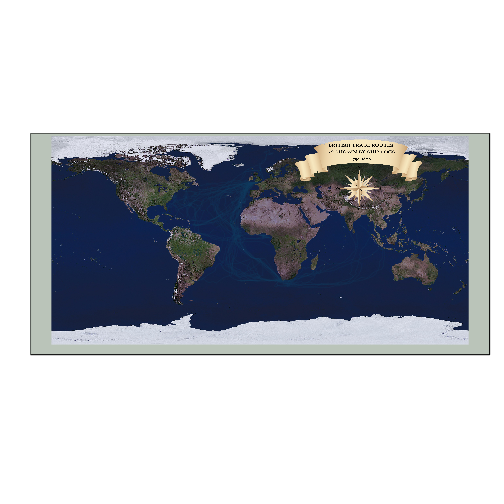
\includegraphics{figure/World_Shipping_with_raster_background.png}
\caption{World Shipping with raster background}
\end{figure}

\subsection{Animating your plots}

R is not designed to produce animated graphics and as such it has very
few functions that enable straightforward animation. To produce animated
graphics users can use a loop to plot and then export a series of images
that can then be stitched together into a video. There are two
approaches to this; the first is to create a loop that fills a folder
with the desired images and then utilise third party software to stitch
the images together, whilst the second uses R's own animation package.
The latter option still requires the installation of an additional
software package called ImageMagick but it has the benefit of creating
the animation for you within R and faciliting the export to a range of
formats, not least HTML and GIF. Here we demonstrate the use of the
package to produce an HTML animation of the shipping tracks completed in
each year of the bdata object. The code snippet below appears extremely
dense, but it only contains a few addtions to the plot code utilised
above.

First load the package:

\begin{Shaded}
\begin{Highlighting}[]
\KeywordTok{library}\NormalTok{(animation)}
\end{Highlighting}
\end{Shaded}
Then clear any previous animation. Obviously the first time you run this
it is unnecessary, but it is a good habit to get into.

\begin{Shaded}
\begin{Highlighting}[]
\KeywordTok{ani.record}\NormalTok{(}\DataTypeTok{reset =} \OtherTok{TRUE}\NormalTok{)}
\end{Highlighting}
\end{Shaded}
We then initiate the ``for loop''. In this case we are using the
\texttt{unique()} function to list the unique years within the
\texttt{bdata} object. The loop will take the first year, in this case
1791, and assign it to the object \texttt{i}. The code inside the
\texttt{\{\}} brackets will then run with \texttt{i=1791}. You will spot
that \texttt{i} is used in a number of places- first to subset the data
when creating the route plot and then as the title in the
\texttt{ggtitle()} function. We need to force ggplot to create the
graphic within the loop so the entire plot call is wrapped in the
\texttt{print()} function. Once the plot is called \texttt{ani.record()}
is used to save the plot still and \texttt{dev.off()} used to clear the
plot window ready for the next iteration. \texttt{i} is then assigned
the next year in the list and the code runs again until all years are
plotted.

\begin{Shaded}
\begin{Highlighting}[]
\NormalTok{for (i in }\KeywordTok{unique}\NormalTok{(bdata$year)) \{}
    \NormalTok{route <- }\KeywordTok{c}\NormalTok{(}\KeywordTok{geom_path}\NormalTok{(}\KeywordTok{aes}\NormalTok{(long, lat, }\DataTypeTok{group =} \KeywordTok{paste}\NormalTok{(trp, group.regroup, }\DataTypeTok{sep =} \StringTok{"."}\NormalTok{)), }
        \DataTypeTok{colour =} \StringTok{"#0F3B5F"}\NormalTok{, }\DataTypeTok{size =} \FloatTok{0.2}\NormalTok{, }\DataTypeTok{data =} \NormalTok{bdata[}\KeywordTok{which}\NormalTok{(bdata$year == i), }
            \NormalTok{], }\DataTypeTok{alpha =} \FloatTok{0.5}\NormalTok{, }\DataTypeTok{lineend =} \StringTok{"round"}\NormalTok{))}
    \KeywordTok{print}\NormalTok{(base + route + wrld + }\KeywordTok{theme}\NormalTok{(}\DataTypeTok{panel.background =} \KeywordTok{element_rect}\NormalTok{(}\DataTypeTok{fill =} \StringTok{"#BAC4B9"}\NormalTok{, }
        \DataTypeTok{colour =} \StringTok{"black"}\NormalTok{)) + }\KeywordTok{annotation_raster}\NormalTok{(btitle, }\DataTypeTok{xmin =} \DecValTok{30}\NormalTok{, }\DataTypeTok{xmax =} \DecValTok{140}\NormalTok{, }
        \DataTypeTok{ymin =} \DecValTok{51}\NormalTok{, }\DataTypeTok{ymax =} \DecValTok{87}\NormalTok{) + }\KeywordTok{annotation_raster}\NormalTok{(compass, }\DataTypeTok{xmin =} \DecValTok{65}\NormalTok{, }\DataTypeTok{xmax =} \DecValTok{105}\NormalTok{, }
        \DataTypeTok{ymin =} \DecValTok{25}\NormalTok{, }\DataTypeTok{ymax =} \DecValTok{65}\NormalTok{) + }\KeywordTok{coord_equal}\NormalTok{() + quiet + }\KeywordTok{ggtitle}\NormalTok{(i))}
    \KeywordTok{ani.record}\NormalTok{()}
    \KeywordTok{dev.off}\NormalTok{()}
\NormalTok{\}}
\end{Highlighting}
\end{Shaded}
The final step in the process is to save the animation to HTML and view
it in your web browser. \texttt{ani.replay()} retrieves the animation
stored by the \texttt{ani.record()} function and
\texttt{outdir = getwd()} ensures the final file is stored in your
working directory.

\begin{Shaded}
\begin{Highlighting}[]
\KeywordTok{saveHTML}\NormalTok{(}\KeywordTok{ani.replay}\NormalTok{(), }\DataTypeTok{img.name =} \StringTok{"record_plot"}\NormalTok{, }\DataTypeTok{outdir =} \KeywordTok{getwd}\NormalTok{())}
\end{Highlighting}
\end{Shaded}
You will note that there is something a little odd about the order in
which the years appear. This can be solved by an additional step before
the loop code above. Have a think then add this in and then regenerate
the animation.

\section{Recap and Conclusions}

This tutorial has covered a large number of techniques and approaches
for the preparation, analysis and visualisation of spatial data in R.
Whilst it only covers the tip of the iceberg in terms of R's
capabilities, it does lay the foundations to the use of the multitude of
other spatial data packages available. These can be discovered online
and through the help documentation and other tutorials provided by the R
community. By utilising the data visualisation techniques and examples
of best practice we have covered it is hoped that you will be able to
communicate your results in a compelling and effective way without the
need for the repetitive ``pointing and clicking'' required of many GIS
packages; you can now tweak colours and other aspects of the plots
without the need to start from scratch each time an iterative
improvement is required. As the R community grows so will its range of
applications and available packages so there will be many exciting
opportunities ahead to improve on what is presented here.

\section{References}

Bivand, R., \& Gebhardt, A. (2000). Implementing functions for spatial
statistical analysis using the language. Journal of Geographical
Systems, 2(3), 307--317.

Bivand, R. S., Pebesma, E. J., \& Rubio, V. G. (2008). Applied spatial
data: analysis with R. Springer.

Burrough, P. A. \& McDonnell, R. A. (1998). Principals of Geographic
Information Systems (revised edition). Clarendon Press, Oxford.

Goodchild, M. F. (2007). Citizens as sensors: the world of volunteered
geography. GeoJournal, 69(4), 211--221.

Harris, R. (2012). A Short Introduction to R.
\href{http://www.social-statistics.org/}{social-statistics.org}.

Kabacoff, R. (2011). R in Action. Manning Publications Co.

Krygier, J. Wood, D. 2011. Making Maps: A Visual Guide to Map Design for
GIS (2nd Ed.). New York: The Guildford Press.

Longley, P., Goodchild, M. F., Maguire, D. J., \& Rhind, D. W. (2005).
Geographic information systems and science. John Wiley \& Sons.

Monkhouse, F.J. and Wilkinson, H. R. 1973. Maps and Diagrams Their
Compilation and Construction (3rd Edition, reprinted with revisions).
London: Methuen \& Co Ltd.

Ramsey, P., \& Dubovsky, D. (2013). Geospatial Software's Open Future.
GeoInformatics, 16(4).

Sherman, G. (2008). Desktop GIS: Mapping the Planet with Open Source
Tools. Pragmatic Bookshelf.

Torfs and Brauer (2012). A (very) short Introduction to R. The
Comprehensive R Archive Network.

Venables, W. N., Smith, D. M., \& Team, R. D. C. (2013). An introduction
to R. The Comprehensive R Archive Network (CRAN). Retrieved from
http://cran.ma.imperial.ac.uk/doc/manuals/r-devel/R-intro.pdf .

Wickham, H. (2009). ggplot2: elegant graphics for data analysis.
Springer.

Wickham, H. 2010. A Layered Grammar of Graphics. American Statistical
Association, Institute of Mathematics Statistics and Interface
Foundation of North America Journal of Computational and Graphical
Statistics. 19, 1: 3-28

\section{Endnotes}

\begin{enumerate}[1.]
\item
  ``What kind of a name is R?'' common question. R's name originates
  from the creators of R, Ross Ihaka and Robert Gentleman. R is an open
  source implementation of the statistical programming language S, so
  its name is also a play on words that makes implicit reference to
  this.
\item
  R is notoriously difficult to search for on major search engines, as
  it is such a common letter with many other uses beyond the name of a
  statistical programming language. This should not be a deterrent, as R
  has a wealth of excellent online resources. To overcome the issue, you
  can either be more specific with the search term (e.g. ``R spatial
  statistics'') or use an R specific search engine such as
  \href{http://www.rseek.org/}{rseek.org}. You can also search of online
  help \emph{from within R} using the command \texttt{RSiteSearch}. E.g.
  \texttt{RSiteSearch("spatial statistics")}. Experiment and see which
  you prefer!
\item
  More information about this ride, and a
  \href{http://www.youtube.com/watch?v=6a8QLiC4LV8\&feature=share}{video}
  from it, can be found on
  \href{http://robinlovelace.net/ecotech/2013/10/13/bicycle-trailer-move.html}{robinlovelace.net}.
\item
  A complete list of drivers for importing and exporting spatial data
  can be displayed by typing \texttt{getGDALDriverNames()}.
\item
  Slots are elements found `inside' classes of the
  \href{http://adv-r.had.co.nz/S4.html}{S4 object system}. While the
  sub-elements of S3 objects such as \texttt{data.frame} are referred to
  using the \texttt{\$} symbol, the slots of S4 objects are identified
  using \texttt{@}. Thus, the variable \texttt{x} of dataframe
  \texttt{df} can be referred to with \texttt{df\$x}. In the same way,
  the data associated with a polygon layer such as \texttt{lnd} can be
  accessed with \texttt{lnd@data}. Note that \texttt{lnd@data} is itself
  a dataframe, so can be further specified, e.g.~with
  \texttt{lnd@data\$name}. For more on spatial data classes, see Bivand
  et al. (2013).
\item
  EPSG stands for ``European Petroleum Survey Group'', but this is not
  really worth knowing as the organisation is now defunct
  (\href{http://www.epsg.org/}{www.epsg.org/}). The important thing is
  that EPSG codes provide a unified way to refer to a wide range of
  coordinate systems, as each CRS has its own epsg code. These can be
  found at the website
  \href{http://spatialreference.org/}{spatialreference.org}. To see how
  this website can be useful, try searching for ``osgb'', for example to
  find the epsg code for the British National Grid.
\item
  To see how the \texttt{crimeAg} dataset was created, please refer to
  the ``Creating-maps-in-R'' tutorial (Cheshire and Lovelace, 2014)
  hosted on
  \href{https://github.com/Robinlovelace/Creating-maps-in-R}{GitHub}.
  The file
  ``\href{https://github.com/Robinlovelace/Creating-maps-in-R/blob/master/intro-spatial-rl.pdf}{intro-spatial-rl.pdf}''
  contains this information, in the section on ``Downloading addtional
  data''.
\end{enumerate}
\begin{Shaded}
\begin{Highlighting}[]
\KeywordTok{source}\NormalTok{(}\StringTok{"chapter.R"}\NormalTok{)  }\CommentTok{# convert chapter to tex}
\end{Highlighting}
\end{Shaded}

\end{document}
